\documentclass[a4paper,12pt]{report}

\usepackage[utf8]{inputenc} % damit auch äöüß gehen
\usepackage[T1]{fontenc}	% so kann man bessere wörtliche rede machen
\usepackage[ngerman]{babel} % deutsche Silbentrennung
\usepackage{SIunits} % SI Einheiten
\usepackage{csvsimple} % for tables
\usepackage{graphicx}
\usepackage{amsmath}
\usepackage{subcaption} % Figures mit mehr als einem Bild
\usepackage{enumitem} % um aufzählungen zu machen
\usepackage[
	colorlinks,
	pdfpagelabels,
	bookmarksopen = true,
	bookmarksnumbered = true,
	linkcolor = black,
	plainpages = false,
	hypertexnames = false,
	citecolor = black
]{hyperref} % verlinkt referenzen für die digitale verwendung

%\renewcommand{\familydefault}{\sfdefault} % NOTE: Hermann liest am Bildschirm lieber serifenlos --hoe


%%% FOR FANCY GRAPHS %%%
\usepackage{tikz}
\usepackage{pgfplots}
\usetikzlibrary{datavisualization}
\usetikzlibrary{datavisualization.formats.functions}

\usepackage{titlepic} % mit Bild auf der Titelseite

%DONE: Einführung - ✓
%DONE: Autor der jeweiligen Funktion - ✓
%DONE: Sinnabschnitte - ✓
%DONE: Literatur/Quellverzeichnis - ✓
%DONE: Gruppenfoto (mit Auto) - ✓
%DONE: Bilder - ✓

%TODO: Passiver Schreibstil
%TODO: Allgemeine Beschreibungen der Kapitel
%TODO: Fazit
%TODO: Zwischenfazit für jedes Kapitel?

\begin{document}

%%%%%%%%%%%%%%%%%%%%% HEADER %%%%%%%%%%%%%%%%%%%%%

	\title{Robotik Praktikum -- Gruppe 2}
	\author{Frauke Jörgens (minf101207) \and Franz Wernicke (ite101729) \and Thorger Dittmann (ite101646) \and Jan Ottmüller (tinf101737) \and Felix Maaß (ite101754)}
	\date{\today}
	\titlepic{\includegraphics[width=\textwidth, height=\textheight, keepaspectratio]{assets/group_photo}}
	\maketitle

	\tableofcontents


%%%%%%%%%%%%%%%%%%%%%%%%%%%%%%%%%%%%%%%%%%%%%%%%%%
\chapter{Einführung}
% Author: Thorger Dittmann

	Begleitend zur Vorlesung ``Einführung in die Robotik'', gehalten von Prof. Dr. Ulrich Hoffmann \cite{hoffmann_ws17}, fand das Robotik-Praktikum statt.
	Ziel war es, die Inhalte der Vorlesung anhand eigener Erfahrungen zu vertiefen und zu lernen, Algorithmen für grundlegende Problemstellungen zu entwickeln.
	Speziell bestand die Aufgabe darin, für ein AADC 2017 Modellfahrzeug eine Programmierung auszuarbeiten.
	Die Idee bestand darin, dass dieses Modellfahrzeug autonom und ohne Kollisionen ein bestimmtes, nicht weiter definiertes Ziel erreicht.
	Im Verlauf des Praktikums sollte man sich daher auch mit den Eigenheiten des vorgegebenen Frameworks auseinandersetzen.

\section{Aufgabenstellung}
% Author: Thorger Dittmann

	Aufgeteilt wurde die Programmierung in Teile mit und ohne Bildanalyse.
	Wir haben uns in der Bildanalyse hauptsächlich mit der Kamerabildauswertung, speziell der Linienerkennung beschäftigt.
	Das Modellfahrzeug sollte einer auf dem Boden abgeklebten ``Straße'' folgen können.
	Im Bereich ohne Bildanalyse wurde sich mit der Sensorik und Aktorik des Fahrzeugs beschäftigt.

\section{Umsetzung im Framework}
% Author: Felix Maaß

	Das uns zur Verfügung gestellte Framework \emph{Automotive Data and Time-Triggered Framework} (kurz: ADTF) der Firma Elektrobit Automotive GmbH\footnote{Weitere Informationen: \url{https://www.elektrobit.com/products/eb-assist/adtf/}} dient zur asynchronen Analyse, Interpretation und Visualisierung von Eingabedaten.
	Daran anknüpfend folgt die Datenausgabe.
	\\
	In unserem Fall sieht dies wie folgt aus:
	\begin{enumerate}
		\item{\textbf{Sensorik:} Erfassen der Umwelt
			\begin{enumerate}
				\item 10x Ultraschallsensoren in verschiedenen Montagewinkeln
				\item 2x Drehimpulsgeber an den Hinterrädern
				\item Intel\textregistered\ RealSense\texttrademark\ R200 Tiefenkamera
				\item Gyroskop, Beschleunigungsmesser und Kompass
				\item Weitwinkel-Rückkamera\footnote{Wird nicht ausgewertet.}
			\end{enumerate}
		}
		\item{\textbf{Logik:} Analyse und Interpretation der Daten
			\begin{enumerate}
				\item Aktuelle Geschwindigkeit und Fahrtrichtung
				\item Hindernis- und Kollisionserkennung
				\item Fahrbahnerkennung
			\end{enumerate}
		}
		\item{\textbf{Aktorik:} Instruktionen an die Hardware
			\begin{enumerate}
				\item Motorsteuerung
				\item Lenksteuerung
				\item Frontscheinwerfer sowie Blink- und Bremslichter
			\end{enumerate}
		}
	\end{enumerate}

\subsection{Konzept der Filter}
% Author: Felix Maaß

	Zur Strukturierung und Modularisierung setzt das ADTF auf sogenannte Filter.
	Dies sind kleine Module, welche aus Inputs, Logik und Outputs bestehen.
	Sie werden in ADTF anschaulich als Blöcke visualisiert (siehe \autoref{img-LaneDetectionConfig}).

	\begin{figure}[ht]
		\centering
		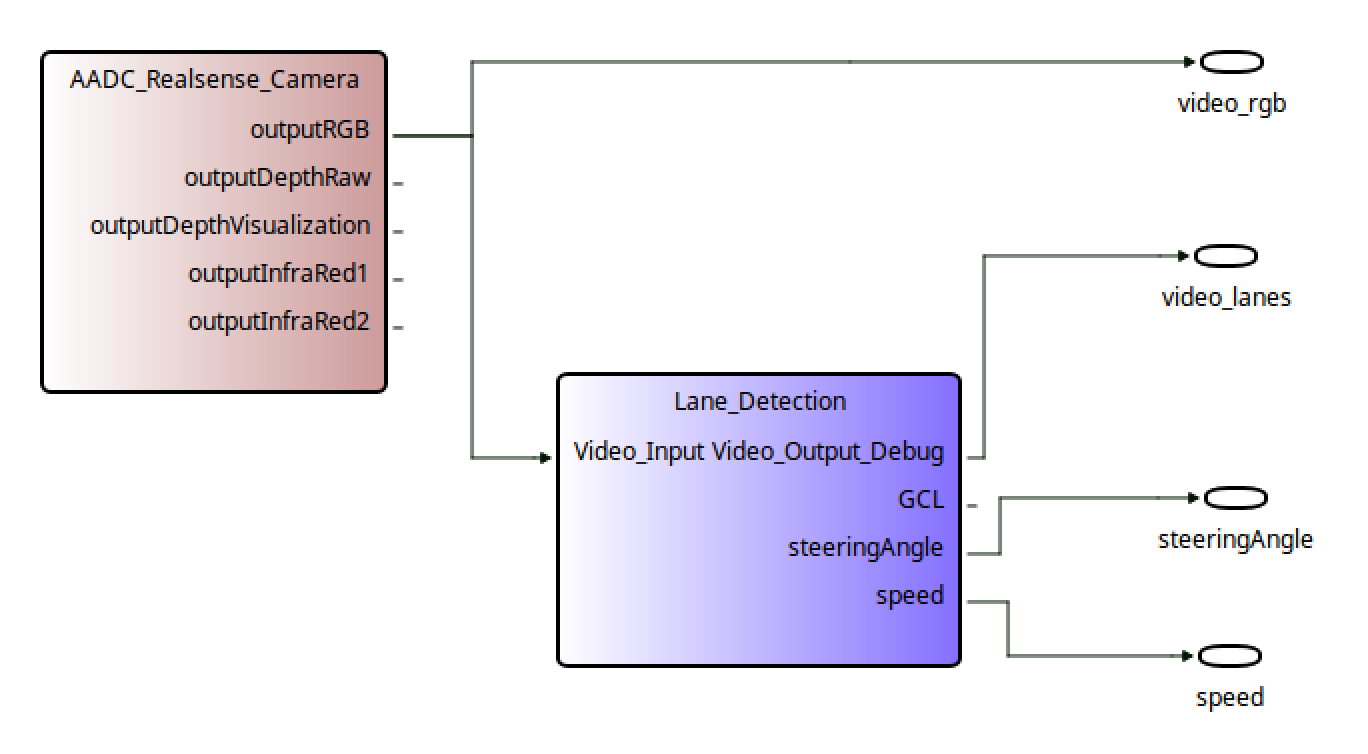
\includegraphics[width=\textwidth, height=\textheight, keepaspectratio]{assets/LaneDetectionConfig}
		\caption{Visualisierung im Konfigurationseditor}
		\label{img-LaneDetectionConfig}
	\end{figure}

	Jedes Modul ist dabei eine \texttt{C++}-Klasse, die die Initialisierung des Blocks und dessen In- und Output-Pins übernimmt.
	Das Modul benachrichtigt, wenn neue Daten an einem Pin anliegen, also zur Verarbeitung zur Verfügung stehen.
	Sodann wird die Logik auf die eingelesenen Daten angewandt und die Ergebnisse über die Outputs wieder nach ``draußen'' gegeben.

	%TODO: Erklärung der FilterProperties?

\subsection{Konzept der Konfigurationen}
% Author: Felix Maaß

	Um Filter zu verwenden, müssen diese in Konfigurationen integriert werden.
	Hier können mehrere Filter gleichzeitig platziert werden.
	Eine erste Konfiguration ist bereits in \autoref{img-LaneDetectionConfig} gezeigt.
	Hier können die durch Filter repräsentierten Logikabschnitte miteinander verbunden werden.
	Die Outputs des einen Filters können dabei also die Inputs des Nächsten darstellen.
	\\
	Dies sieht dann zum Beispiel so aus:\footnote{Visualisiert in \autoref{img-LiveConfig}.}
	\begin{enumerate}
		\item Arduino triggert und liest Ultraschallsensoren aus.
		\item Daten stehen der Hinderniserkennung (siehe \autoref{section-ObstacleDetection}) zur Verfügung.
		\item Motorregler erhält ``Hindernis erkannt''-Signal und leitet Nothalt ein.
		\item Arduino stoppt die Motoren.
	\end{enumerate}

	Um Filter miteinander verbinden zu können, muss die Typkompatibilität gewährleistet sein.
	So ist es zum Beispiel nicht möglich, einen Wahrheitswert an einen Eingang weiterzugeben, der eine Fließkommazahl erwartet.

\subsubsection{Verschachtelung}
% Author: Felix Maaß

	Ebenso ist es möglich, Konfigurationen in Anderen einzubetten, sie also zu verschachteln.
	In unserer ``Live''-Konfiguration (siehe \autoref{img-LiveConfig}) wurde die Fahrbahnerkennung, die zur Übersichtlichkeit eine eigene Konfiguration besitzt, eingebettet.
	Darüber hinaus wurden auch die Filter, die für Low-Level-Operationen zuständig sind, in die ``Main''-Konfiguration ausgelagert.

	\begin{figure}[ht]
		\centering
		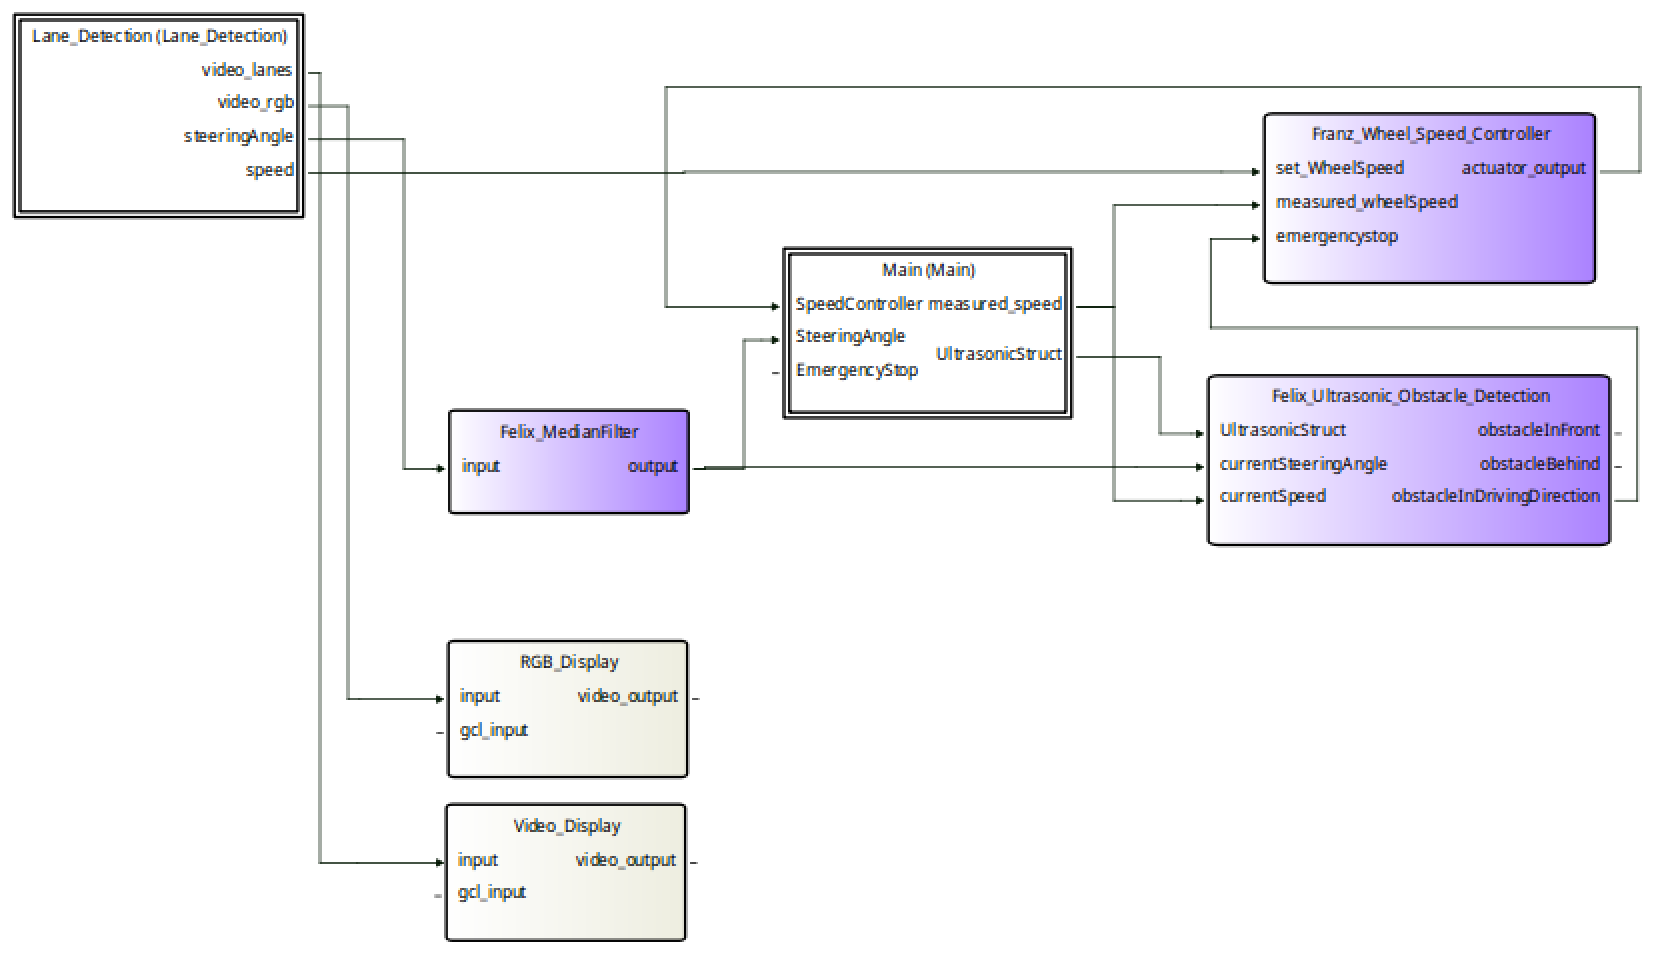
\includegraphics[width=\textwidth, height=\textheight, keepaspectratio]{assets/LiveConfig}
		\caption{Verschachtelungen von Konfigurationen}
		\label{img-LiveConfig}
	\end{figure}

%%%%%%%%%%%%%%%%%%%%%%%%%%%%%%%%%%%%%%%%%%%%%%%%%%
\chapter{Allgemeine Themen}
\section{Standard-Filter}
% Author: Felix Maaß

	Um einen ADTF-Filter zu implementieren, muss viel Code geschrieben werden, bevor man überhaupt mit der wirklichen Logik anfangen kann. %NOTE: bessere formulierung finden --felix
	Um uns diesen Schritt zu vereinfachen, wurde eine abstrakte Klasse \texttt{cStdFilter} erstellt, die von der vorgegebenen Klasse \texttt{cFilter} erbte.
	Sie bot uns Standard-Implementationen sowie Hilfsroutinen und vermied somit Redundanzen über die ganze Code-Basis.
	Dadurch ließen sich im Durchschnitt etwa 170 Zeilen Code pro Filter sparen.
	Der jedoch größte Gewinn bestand darin, dass Korrekturen und Implementationen weiterer Hilfsfunktionen so nur einmal an einer zentralen Stelle durchzuführen waren und dadurch eine höhere Übersichtlichkeit gewährleistet wurde.

\section{Lineare Funktion}
% Author: Felix Maaß

% TODO: Diese Sektion muss irgendwo einsortiert werden oder braucht eine eigene Einleitung "es gibt im system viele messwerte, die als einfache Fließkommazahlen…" --hoe

	Für manche Werte war es nötig eine Modulation hinzufügen zu können.

	Es wurde sich aus Gründen der besseren Visualisierung für einen eigenen ADTF-Filter entschieden.
	Dieser nimmt ein Eingangssignal entgegen, welches daraufhin mit einem Gain und Offset versehen wird und anschließend den modulierten Wert zurückliefert.

	Diese Funktionalität entspricht einer ``Linearen Funktion'':

	\[y = g \cdot x + o\]

	wobei $x$ der Eingang, $g$ der Gain, $o$ der Offset und $y$ der Ausgang ist.
	\\
	Gain und Offset können hierbei sowohl über eigene Eingangspins als auch über variable Filterparameter gesetzt werden.


\section{Float Wert Generator}
% Author: Franz Wernicke

	Um verschiedene Filter zu testen, die einen Wert als Eingang benötigten, wurde dieser Block erstellt.

	Da neue Ausgaben nur durch die Methode \texttt{OnPinEvent} ausgelöst wurden, definierten wir einen \texttt{WatchDog} als Input. So wird mit jedem Auslösen des WatchDog der Wert gesendet. Der Wert kann in den Einstellungen des Filters während der Laufzeit gesetzt werden.


\subsection{In Entwicklung}

	Es ist geplant, dass die Geschwindigkeit des Autos mithilfe des aktuellen Lenkwinkels in Kurven angepasst werden kann.

%%%%%%%%%%%%%%%%%%%%%%%%%%%%%%%%%%%%%%%%%%%%%%%%%%
\chapter{Lenkung}
% Autor: Felix Maaß

	Dieses Kapitel befasst sich mit der Ansteuerung des Lenkservomotors und den dabei aufgetretenen Schwierigkeiten.
	Es existiert bereits eine vorgefertigte Implementation eines Filters, welcher sich um die Kommunikation mit den Arduinos kümmert.
	Standardmäßig erwartet dieser Arduino-Controller einen Wert zwischen $-100$ und $+100$, um den Servomotor für die Lenkung richtig zu instruieren.

	Es wurde eine Modularisierung eingeführt, die das Vorhaben der Ansteuerung in die im folgenden beschriebenen Bereiche aufteilt.

\section{Mittels Winkel}
\label{Steering-Angle-To-Servo}

	Die erste Abstraktionsebene stellt das Mapping von Lenkwinkel zu Servostellung dar.
	Hierfür ist es nötig zu wissen, welchen Wert der physikalisch bedingte, maximale Lenkwinkel hat.

	Wir stellten fest, dass die Auslenkung der Vorderräder unterschiedlich stark erfolgt.
	Dies liegt daran, dass die Räder unterschiedlichen Radien folgen müssen, um einen gemeinsamen Kurvenmittelpunkt zu besitzen.
	Gibt es keinen Gemeinsamen, so entsteht mehr Abrieb bzw. Schlupf, was wiederum zu ungenauen Lenk- und Wegverhalten führt.

	Oft verwendet wird die sogenannte Ackerman-Lenkung \cite{berry16}, die genau diesem Prozess entgegenwirken soll, indem die Räder unterschiedlich stark einlenken.

	\paragraph{Theorie.}
	Es wurde sich für eine Annäherung der Winkel entschieden, da wir die Räder nicht getrennt anstellen können.
	Wir denken uns idealisiert ein Rad in der Mitte der Vorderachse und führen unsere Berechnungen anhand dessen durch.

	\begin{figure}[ht]
		\centering
		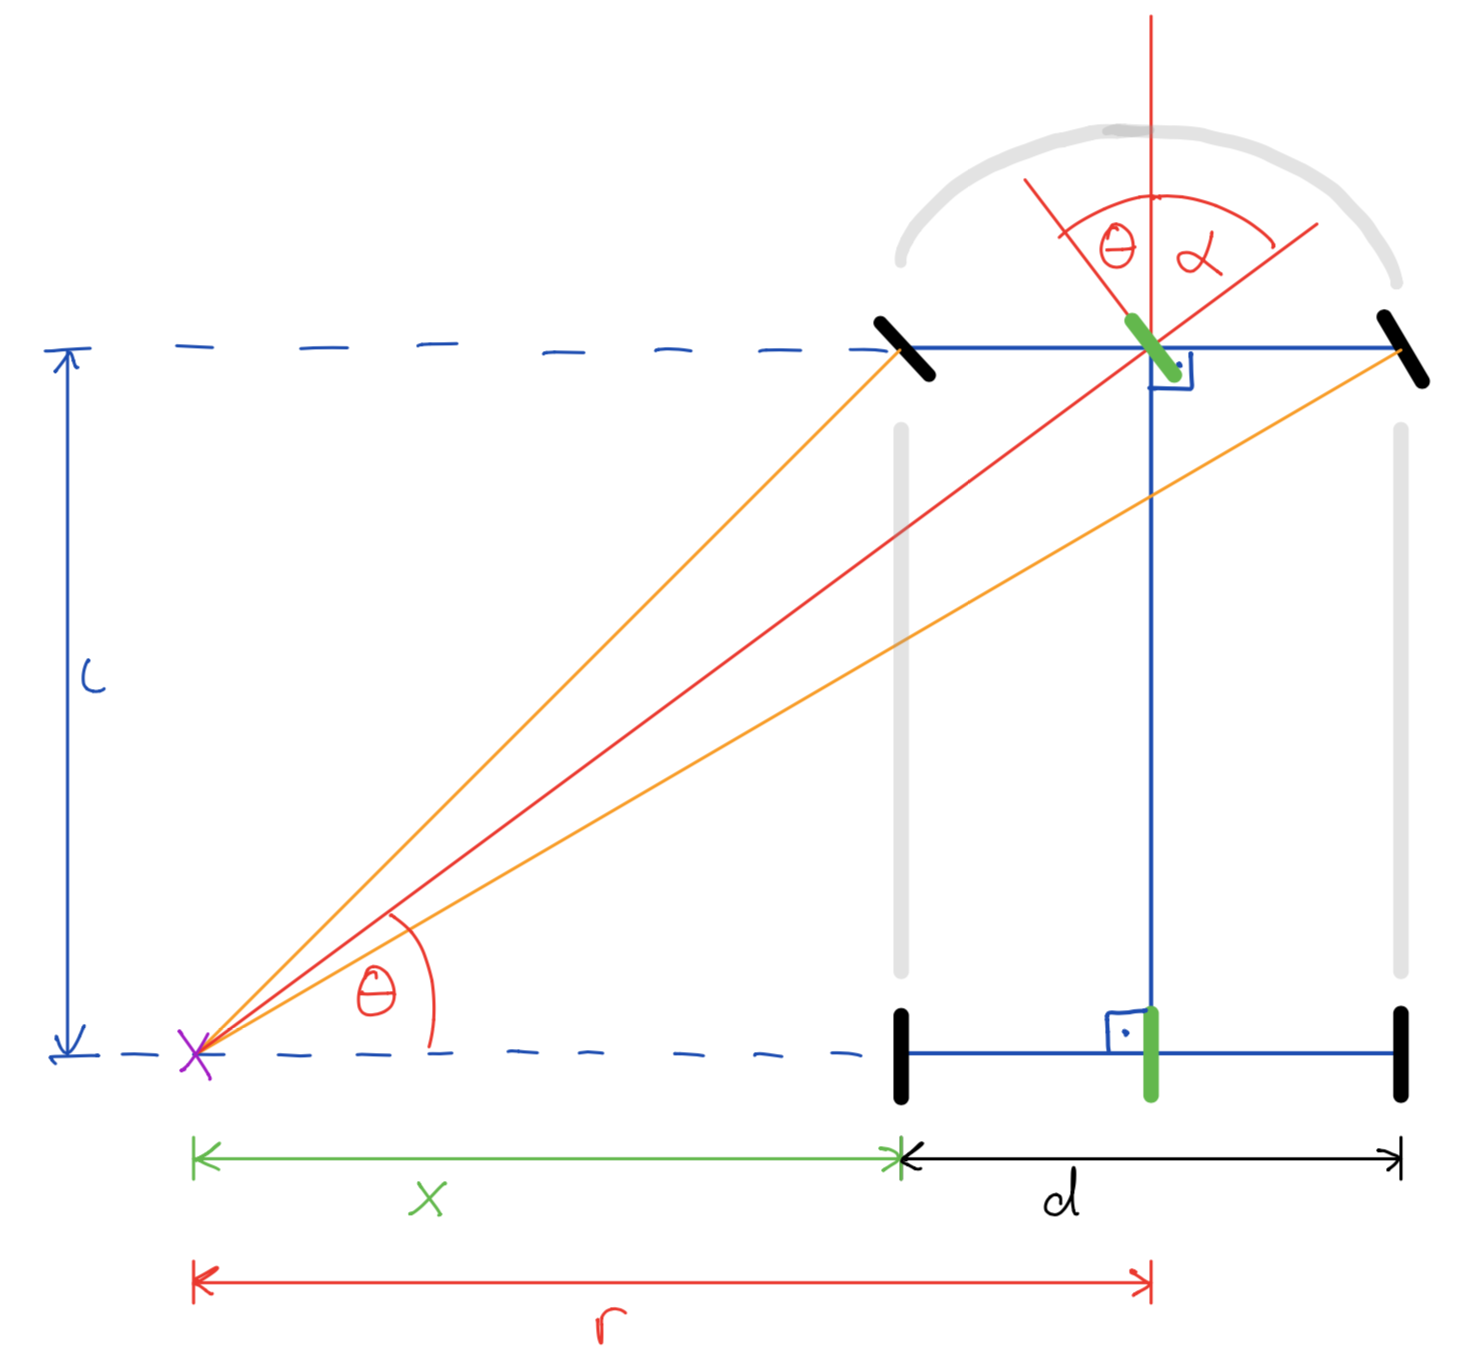
\includegraphics[width=\textwidth,height=\textheight,keepaspectratio]{assets/Lenkwinkel-Skizze.png}
		\caption{Skizze des idealisierten Lenkwinkels}
		\label{img-steering-angles-sketch}
	\end{figure}
	\pagebreak

	Basierend auf den in \autoref{img-steering-angles-sketch} skizzierten trigonometrischen Überlegungen wurde folgende Gleichung entwickelt:

	\begin{align*}
		&&\theta_{max} &= \arctan\left( \frac{l}{r} \right)\\
		&&&= \arctan\left( \frac{l}{x_{min} + \frac{d}{2}} \right) &&\|\quad d = 260mm, l = 360mm
	\end{align*}
	\\
	Hierbei stellt $d$ die Spurweite und $l$ den Radstand dar.

	Aufgrund des Schlupfes erwiesen sich theoretische Werte für den minimalen Innenradius $x_{min}$ nicht als akkurat, weshalb dieser sodann durch  Praxistests % NOTE: Falls noch vorhanden, Rohdaten gerne als Anhang beilegen (eingescannter Zettel reicht mir schon) --hoe
	empirisch ermittelt wurde:
		\[x_{min} = 400mm.\]

	\paragraph{Resultat.}
	Dieses Vorgehen generierte eine zufriedenstellende Lösung.
	Der maximale Lenkwinkel wurde zu $\theta_{max} \simeq 34,19\degree$ bestimmt.

	Es erfolgt eine Übersetzung des gewünschten Lenkwinkels von $-\theta_{max}$ bis $+\theta_{max}$ auf die nötigen Servoansteuerungswerte zwischen $-100$ und $100$.

\section{Mittels Radius}

	Die zweite Abstraktionsebene stellt den Übergang von von Kurvenradius zu Lenkwinkel dar.
	Einige notwendige Vorkenntnisse sind bereits in \autoref{Steering-Angle-To-Servo} erläutert worden.
	Darauf setzt dieser Filter nun wie folgt auf:

		\begin{align*}
		&&\theta\left(r\right) &= \arctan\left( \frac{l}{r} \right)\\
		&&&= \arctan\left( \frac{l}{r - \frac{d}{2}} \right) &&\|\quad d = 260mm, l = 360mm
		\end{align*}

	Analog zu \autoref{Steering-Angle-To-Servo} stellt $d$ die Spurweite und $l$ den Radstand dar.

	\paragraph{Resultat.}
	Soll nun ein bestimmter Kurvenradius eingestellt werden, wird der dazugehörige Winkel berechnet und daraufhin zum Servowert umgerechnet.

% TODO: Bemerken, dass sowas in ADTF schon drin ist und begründen, warum deren Filter nicht verwendet wurde. --hoe

%%%%%%%%%%%%%%%%%%%%%%%%%%%%%%%%%%%%%%%%%%%%%%%%%%
\chapter{Motorregelung}
% Author: Franz Wernicke

	Die Geschwindigkeit sollte in \meter\per\second\usk angegeben werden.
	Da die Arduinos nur Werte zwischen $-100$ und $+100$ annehmen, musste dies zunächst umgerechnet werden.
	Zusätzlich sollte die Geschwindigkeit geregelt werden, um bei verschiedenen Fahrtzuständen immer die Sollgeschwindigkeit zu erreichen.

	Über Drehimpulsgeber wird die zurückgelegte Strecke ermittelt.
	Ein Ableiten nach der Zeit liefert die Geschwindigkeit.

	Im ADTF sind bereits zwei nutzbare Filter vorhanden:
	\begin{enumerate}[label=]
		\item Converter Wheels, der die Werte der Wheel Encoder in eine Geschwindigkeit umrechnet.
		\item Wheel Speed Controller, welcher verschiedene Regelalgorithemen darstellt.
	\end{enumerate}
	Die fertigen Filter boten bereits einen guten Ausgangspunkt und wurden zunächst übernommen.
	Um einen guten Regler zu erhalten, sollte zuerst das System des Autos bestimmt werden.
	Dazu sollte eine Sprungfunktion aufgenommen werden.
	Dies erwies sich als schwieriger als erwartet, da das Auto eine recht hohe Endgeschwindigkeit besaß und der Boden in der Robotik und in dem Flur davor sich als sehr rutschig herausstellte.

	Nach einigen Überlegungen fiel die Wahl der Teststrecke auf den Flur vor dem Rechnernetzelabor.
	Dieser war sehr lang, eben und bietete direkt vor der Tür des Labors eine Fußmatte, die durch bessere Traktion eine hohe Beschleunigung erlaubte.

\section{Aufnahme der Sprungfunktion}
	Durch den \emph{HardDisk-Recorder} konnten die Sensorwerte auf einfache Weise aufgenommen werden.
	Die Aufgabe bestand sodann darin, dass Auto sprungfunktionsartig zu Beschleunigen.

	Auf dem Weg zur Teststrecke wurde der geräumigen Flur vor Hörsaal 5 genutzt, um einen Test durchzuführen und auch diesen aufzuzeichnen.

	Zur Auswertung der Messdaten wurde der \emph{Wheel Speed Converter} angepasst, um die Messwerte in eine CSV Datei zu schreiben.
	Diese CSV Datei wurde dann in einer Tabellenkalkulation bearbeitet.

	Zuerst wurde bestimmt, wann die Beschleunigung beginnt und wann die Höchstgeschwindigkeit erreicht ist.
	Alle Werte vor und nach diesem Zeitraum wurden entfernt.
	Da die Zeitstempel die ganze Zeit mitlaufen, mussten die Zeiten auf den Anfang der Beschleunigung verschoben werden.
	Durch diese Anpassungen erhielten wir die Graphen \ref{img-accelleration1} und \ref{img-accelleration2}.
	\begin{figure}[ht]
		\centering
		\begin{tikzpicture}
		\begin{axis} [xlabel=Zeit in \second, ylabel=Geschwindigkeit in \meter\per\second]
		\addplot+ table [x=Time, y=Speed, col sep=semicolon, mark=none] {../Speed Controller/speedValue_Acceleration1.CSV};
		\end{axis}
		\end{tikzpicture}

		\caption{Beschleunigung vor HS5}
		\label{img-accelleration1}
	\end{figure}

	%DONE: Display units on axis values like  m/s : https://tex.stackexchange.com/questions/126188/how-do-i-set-units-in-pgfplots-without-square-brackets#126189
	\begin{figure}[ht]
		\centering
		\begin{tikzpicture}
		\begin{axis} [xlabel=Zeit in \second, ylabel=Geschwindigkeit in \meter\per\second]
		\addplot+ table [x=Time, y=Speed, col sep=semicolon, mark=none] {../Speed Controller/speedValue_Acceleration2.CSV};
		\end{axis}
		\end{tikzpicture}

		\caption{Beschleunigung vor RN-Labor}
		\label{img-accelleration2}
	\end{figure}

	\paragraph{Auswertung}
	Als Höchstgeschwindigkeit wurde ein Mittel der höchsten Geschwindigkeitswerte genommen.
	Dazu wurden die Werte betrachtet und mithilfe von verschieden breiten Medianen die Werte gefiltert.
	Nun wurden die Differenzen betrachtet.
	Durch die Messungenauigkeiten kam es immer wieder zu negativen Differenzen.
	Daher wurden alle Werte, wonach die Differenz weniger als 1\% der aktuellen Geschwindigkeit besaß, als erreichte Höchstgeschwindigkeit interpretiert.

	Die erste Beschleunigung diente nur als Test, um ein Gefühl für das Fahrverhalten des Autos bei höheren Geschwindigkeiten zu bekommen, bevor der eigentliche Test im deutlich engeren Flur durchgeführt wurde.
	So wurden auch schon die Höchstgeschwindigkeit und die dafür benötigte Strecke abgeschätzt.

	Aus der zweiten Beschleunigung ermittelten wir eine Höchstgeschwindigkeit von $4,75 \meter\per\second$.
	\begin{figure}[ht]
		\centering
		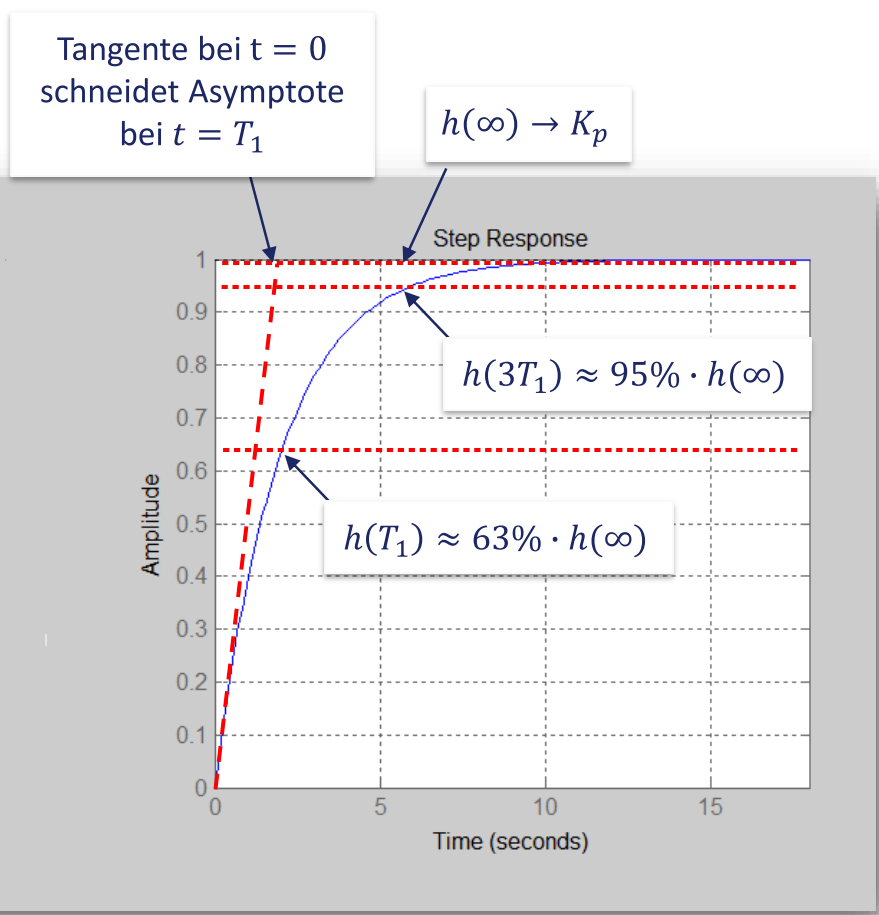
\includegraphics[width=250pt,keepaspectratio]{assets/PT1-Sprungantwort.PNG}
		\caption{Sprungantwort eines PT1 Gliedes \cite{Regelungstechnik}}
		\label{img-PT1-Sprungantwort}
	\end{figure}\\
	Wird unser Graph mit dem Graph aus der Grafik \ref{img-PT1-Sprungantwort} verglichen, liegt es nahe, dass sich das Auto wie ein PT1-Glied verhält. Daher sind wir von einem $PT_1$-Glied ausgegangen. \\
	Wie in \autoref{img-PT1-Sprungantwort} gezeigt, ließen sich dann die Werte des Gliedes bestimmen.\\
	So wurde bei unserem Auto $K_p$ mit $5,75 \meter\per\second\usk$ und $T_1$ mit $0,5\second\usk$ ermittelt.\\

	\paragraph{Bestimmen der Regelparameter}
	\begin{figure}[ht]
		\centering
		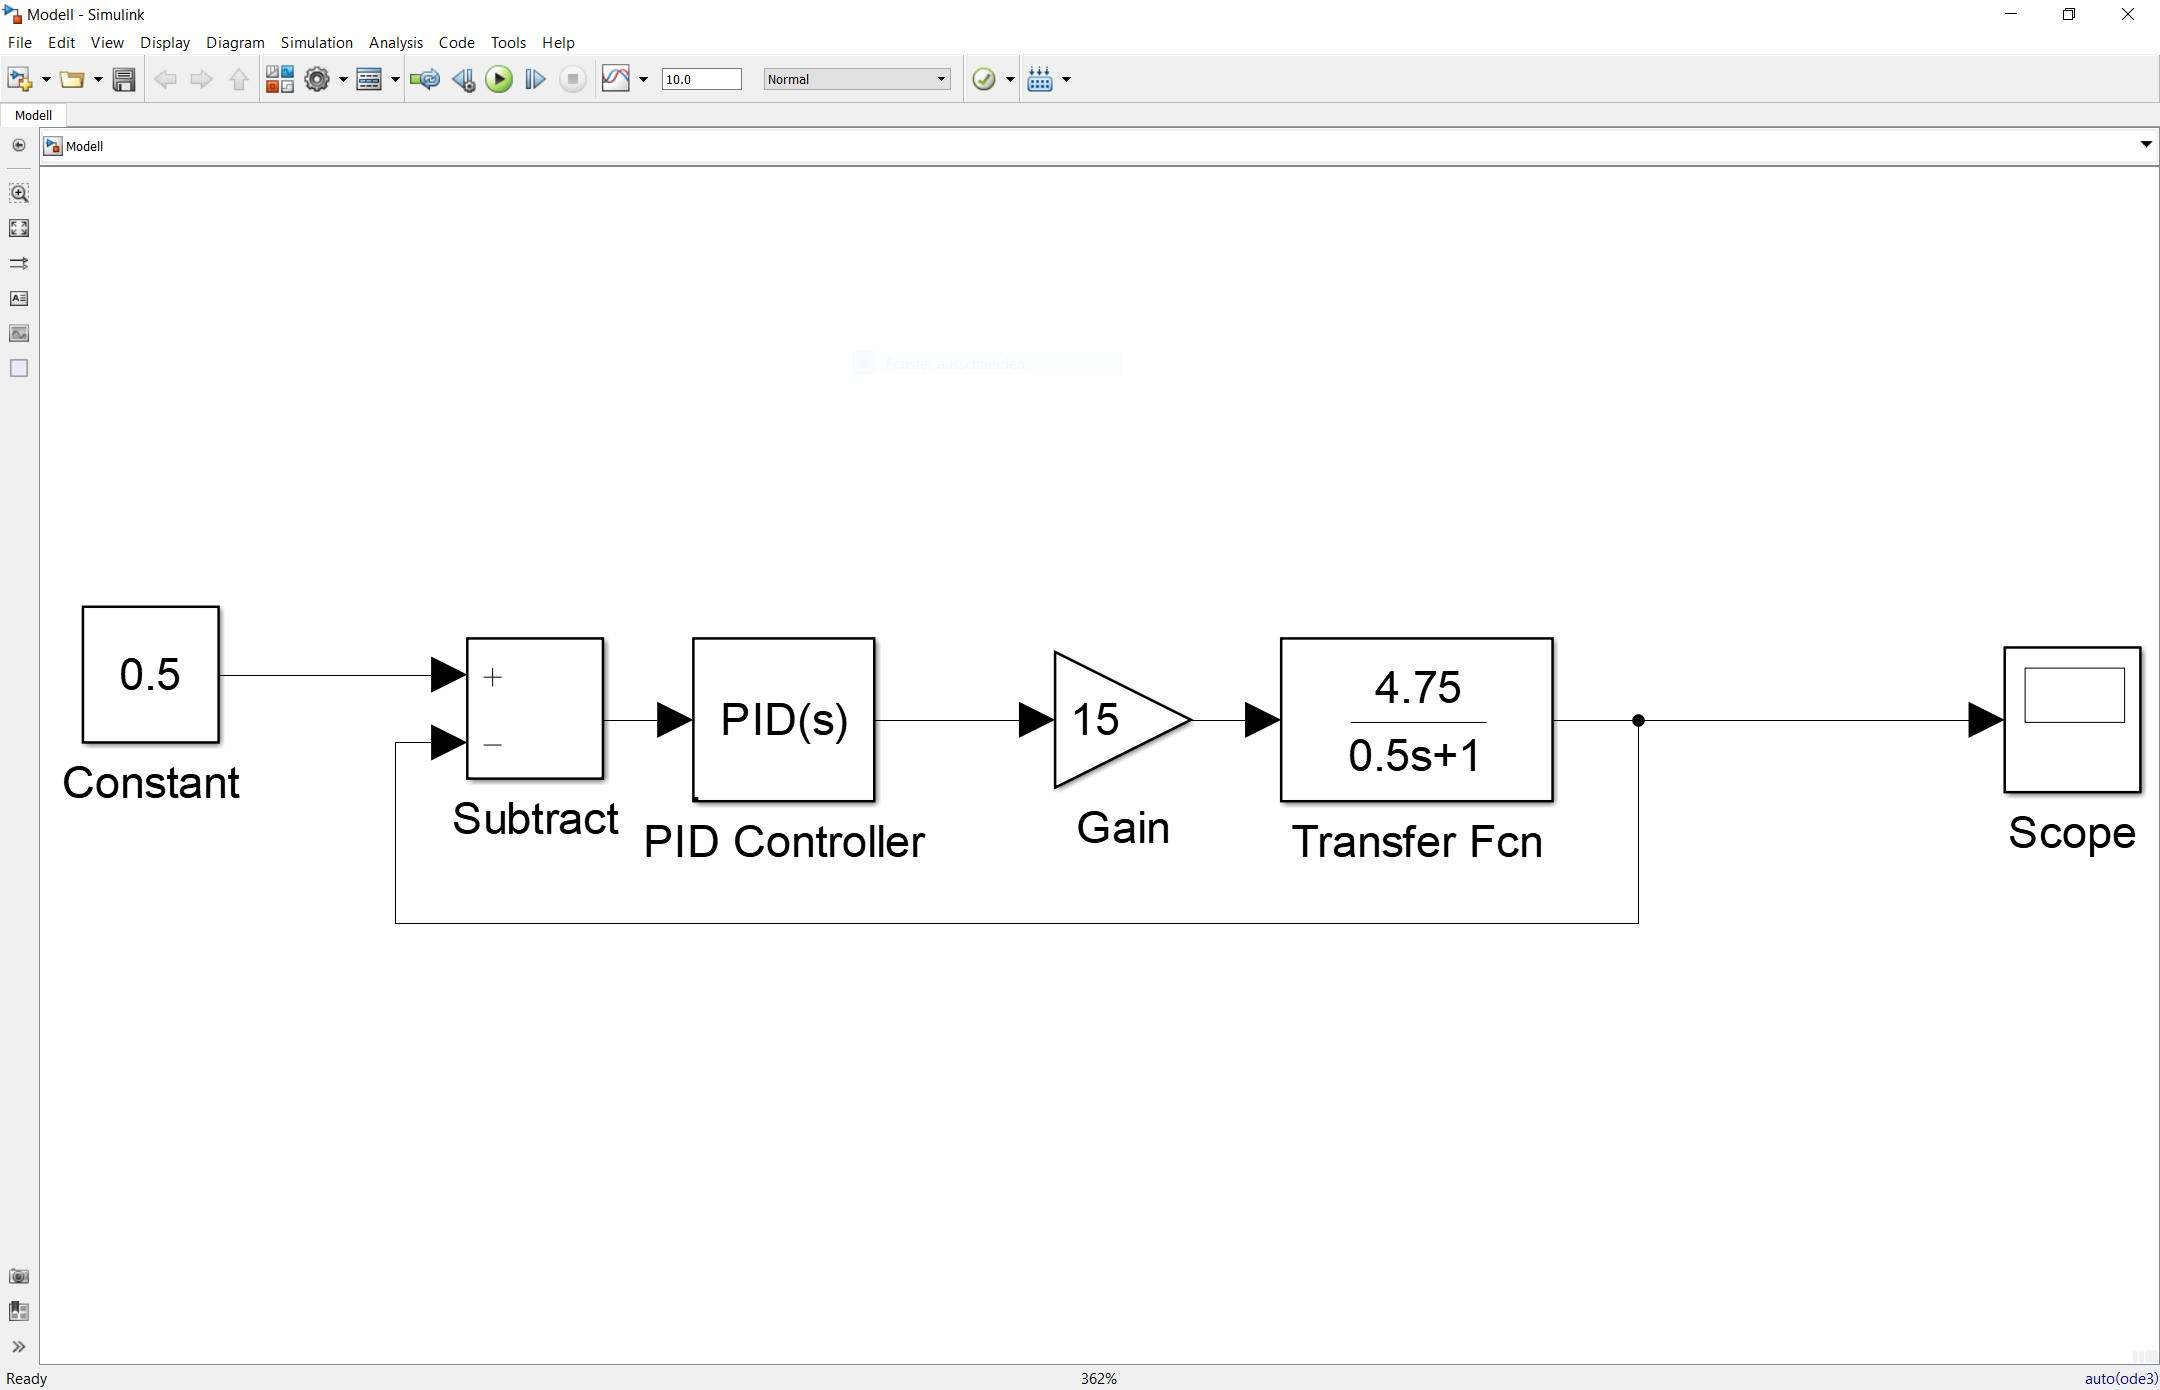
\includegraphics[width=250pt,keepaspectratio]{assets/Simulink.PNG}
		\caption{Das System in Simulink}
		\label{img-Simulink}
	\end{figure}

	\begin{figure}[ht]
		\centering
		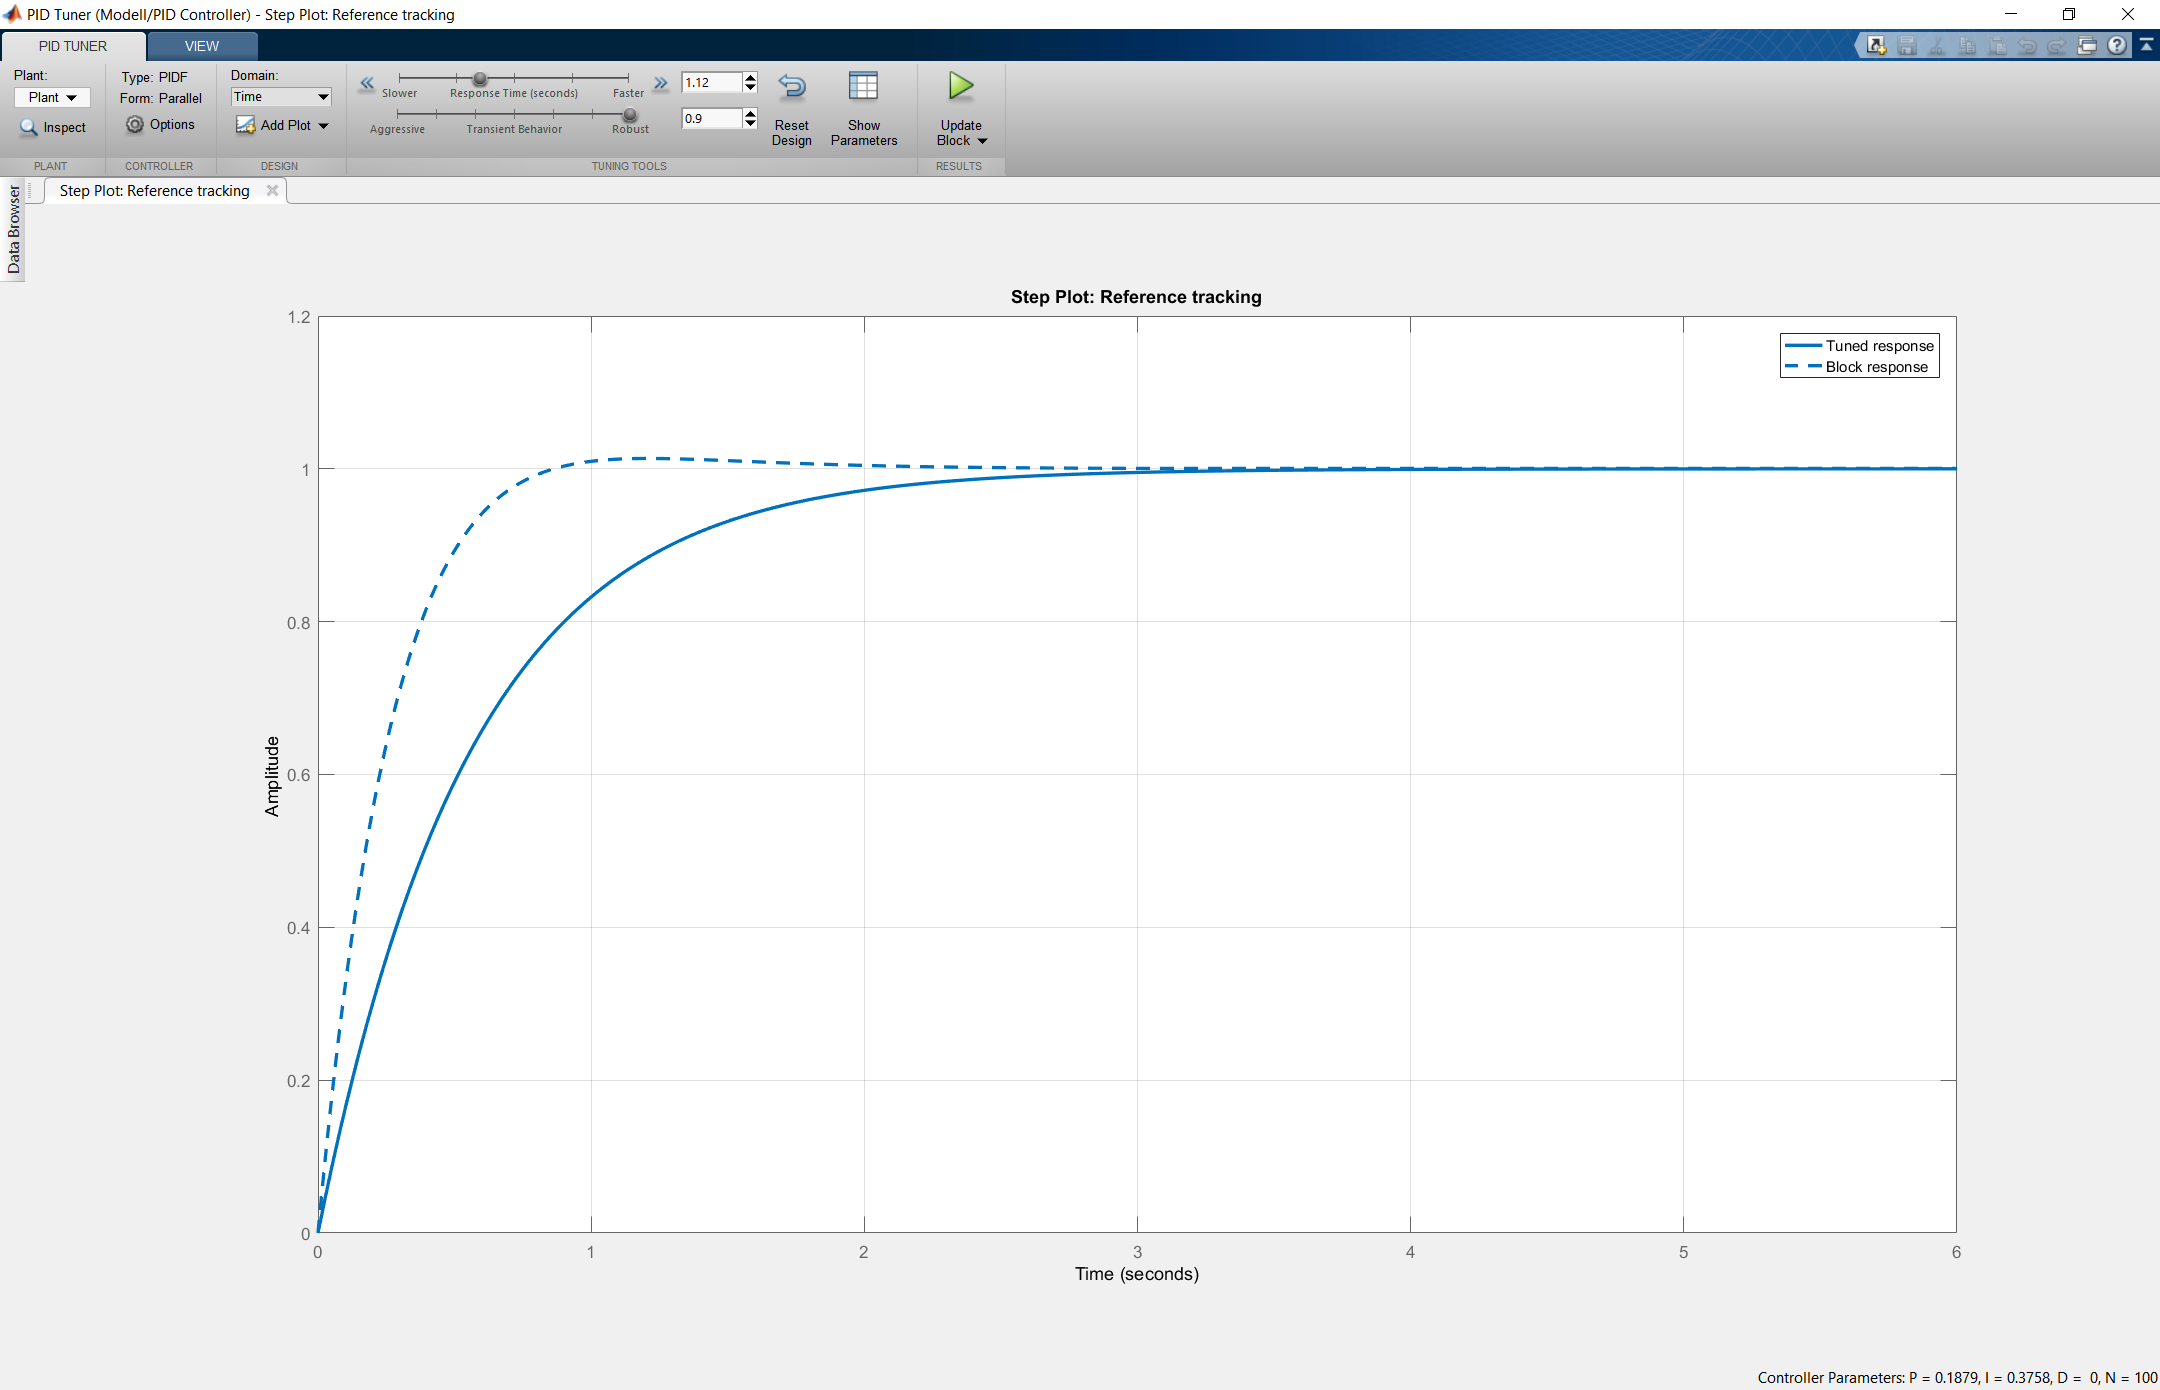
\includegraphics[width=250pt,keepaspectratio]{assets/PID-Tuner.PNG}
		\caption{PID-Tuner in Simulink}
		\label{img-PID-Tuner}
	\end{figure}

	Die ermittelten Systemparameter wurden in Simulink in eingegeben (siehe \autoref{img-Simulink}). \\
	Das System konnte so dann bei weiteren Untersuchungen auch simuliert werden. \\
	Mit dem \emph{PID-Tuner} (\autoref{img-PID-Tuner}) wurden dann Werte für den PID Regler bestimmt.
	Die so ermittelten Werte betrugen dann: \\
	\begin{gather*}
		K_{PR} = 0.39088 \\
		K_{IR} = 0.98867 \\
		K_{DR} = 0.01398 \\
		\text{für einen parallelen PID-Regler der Form}\\
		y(t) = K_{PR} \cdot e(t) + K_{IR} \cdot \int_{0}^{t} e(t)dt + K_{DR} \cdot \frac{de(t)}{dt}
	\end{gather*}
	Die so bestimmten Werte wurden dann mit dem Auto im Praxistest ausprobiert.
	Dabei wurde festgestellt, dass das Auto viel langsamer beschleunigte, als die Simulation in Simulink es vermuten lies.
	Wir nehmen an, dass das System eine höhere Dämpfung besitzt als zuerst vermutet.
	Um diesem entgegen zu wirken wurde ein zusätzlicher Gain hinter den eigentlichen Regler geschaltet.
	Da die Werte in dem Regler mit hoher Genauigkeit verarbeitet werden (\texttt{float64}), kann die Ausgabe mit einem Gain versehen werden, ohne dass die Reglung zu stark diskretisiert wird, was wieder zu neuen Problemen führen würde.
	Mit diesem lies sich nun die Geschwindigkeit des Reglers weiter anpassen.
	Durch probieren hatte sich im Vorfeld herausgestellt, dass das Auto ab einem Ausgabewert von 8 Anfährt.
	Durch debug Ausgaben wurde festgestellt, dass der Regler mit Ausgaben etwa eine Potenz unter diesem Wert lag.
	So wurde als Übergangslösung ein Gain von 10 verwendet
	 Da dies immer noch etwas langsam war, wurde Gain auf 15 erhöht. \\

\section{Bremslichter}
	Es sollten bei Bremsmanövern die Bremsleuchten eingeschaltet werden.
	Ein erster Ansatz ist es im Stand und bei stärkerer Verzögerung die Bremsleuchten einzuschalten.
	Der erste Teil konnte einfach umgesetzt werden, so wurden beim Zurücksetzen des Reglers die Bremsleuchten eingeschaltet.
	Das beschleunigungs-abhängige Einschalten war schwieriger, da durch Messungenauigkeiten und Schwingungen im Regler der Ausgabewert bei normaler Fahrt stärker schwankt als beim Bremsen.
	Es wurden Schwankungen im Output bei normaler Fahrt von etwa $1$ beobachtet, während beim Bremsen der Output sehr kontrolliert verringert wird, etwa $0.1$ pro Berechnung.

\section{Probleme mit dem ADTF}
	Die Arbeit mit den vorimplementierten Filtern von ADTF stellte sich als schwierig heraus. \\
	Es wurde versucht die Qualität der Filter zu ermitteln.
	Zuerst wurde der \texttt{AADC Wheel Speed Converter} untersucht. \\
	Dazu wurde zuerst der Motor mit dem \texttt{AADC Car Controller} angesteuert und die Geschwindigkeitsausgabe des \texttt{AADC Wheel Speed Converter} in ein \texttt{Scope Display} geleitet.
	Dabei wurde festgestellt, dass bei augenscheinlich proportional wachsender Geschwindigkeit auf dem \texttt{Scope Display} die Werte exponentiell zunahmen.
	Dieses Verhalten überraschte sehr, so wurde danach die zurückgelegte Strecke angezeigt.
	Auch hier wurde bei konstanter Geschwindigkeit ein exponentiell wachsender Wert beobachtet.
	Aufgrund dieses Verhaltens wurde das \texttt{Table Display} verwendet.
	Hier stellte sich heraus, das dieses jeweils \emph{8 Bit} der Eingabe in einem Feld darstellt, so konnte diese Ansicht auch nicht verwendet werden.
	Um die Werte beurteilen zu können musste also die Klasse \texttt{cConverterWheels} angepasst werden, sodass die berechneten Werte dann in die Konsole geschrieben wurden. \\
	Danach wurde auch der \texttt{AADC Wheel Speed Controller} getestet.
	Dieser funktionierte bereits in einem zufriedenstellend Maße.
	Bei betrachten des Codes des Filters wurde jedoch sehr viel redundanter Code gefunden.
	So wurde für einen PID Regler, jede einfachere Variante einzeln implementiert, also für P, PI und PID.
	Diese Redundanz wurde zuerst entfernt, um die Übersichtlichkeit zu verbessern.
	Zusätzlich wurden noch Debug Ausgaben hinzugefügt um die korrekte Arbeit des Reglers nachzuvollziehen. \\


%%%%%%%%%%%%%%%%%%%%%%%%%%%%%%%%%%%%%%%%%%%%%%%%%%
\chapter{Kollisionsvermeidung}
% Author: Felix Maaß

	Mithilfe der Ultraschallsensoren waren vorn und hinten Hindernisse zu erkennen.
	Dadurch sollte es möglich sein zu reagieren, bevor eine Kollision stattfand.

\section{Genauigkeit der Ultraschallsensoren}

	\paragraph{Situation.}
	Die Ultraschallsensoren lieferten einzeln betrachtet recht akkurate Werte.
	Die Genauigkeit wurde zu $\pm1cm$ bestimmt.

	\paragraph{Problem.}
	Leider war es jedoch der Fall, dass die Messungen Ausreißer aufwiesen.
	Teils wurden leicht erkennbare Fehler zurückgegeben ($-1$), teils wichen die Werte aber auch um erhebliche Beträge ab.

	Den Grund für Letzteres diagnostizierten wir in der gleichzeitigen Ansteuerung der Sensoren.
	Da jedoch der Code der Arduinos (welche sich um die Erfassung der Werte kümmern) nicht offen lag, konnten wir vorerst keine Änderungen daran vornehmen.

	Damit diese falschen Werte dennoch nicht mit in kommende Berechnungen einbezogen wurden, musste eine entsprechende Lösung gefunden werden.

	\paragraph{Maßnahme.}
	Zur Stabilisierung der Messwerte entschieden wir uns für eine Filterung.
	Es wurde nach einem Filter gesucht, der robust gegenüber Ausreißern ist.
	Hier kam als Erstes ein Medianfilter in den Sinn.

	Ein entsprechender Filter wurde nun sowohl als C++ Klasse als auch als ADTF-Filter erstellt.

	Der ADTF-Filter besitzt einen Parameter, der die Fenstergröße einstellt (i.e. die Anzahl an Werten über die der Median gebildet werden soll) und ermöglicht damit eine flexible Filterung der Messwerte.

\section{Hinderniserkennung}
\label{section-ObstacleDetection}

	Mithilfe der aufbereiteten Ultraschallsensordaten wird es möglich sein, das Auto sicher durch die Umgebung zu navigieren.\footnote{Dieses Feature befindet sich noch in Entwicklung.}

\subsection{Theoretische Überlegungen}

	Um sich ein geeignetes Bild der Umgebung zu machen, ist es sinnvoll, jeden  Messwert der fünf Frontsensoren einzeln zu bewerten, da sonst unnötige Manöver ausgeführt werden, um Objekten auszuweichen, die nicht auf unserer Trajektorie liegen.
	Uns erschien es sinnig, dies anhand des aktuellen Lenkwinkels und der Geschwindigkeit zu tun.

\subsubsection{Glockenkurve}

	Es wurde eine Funktion synthetisiert, die die Relevanz der einzelnen Messwerte zu dem Lenkwinkel in Relation setzt:

	\begin{align*}
		y=\frac{2}{\sqrt{b}} - e^{-3b \cdot \left( x-\alpha \right)^2}
		&&||\quad b=
		\begin{cases}
			1,					& \text{wenn } v \leq v_{std} \\
			\frac{16}{9},		& \text{wenn } v \geq \frac{16}{9} \cdot v_{std} \\
			\frac{v}{v_{std}}, 	& \text{andernfalls}
		\end{cases}
	\end{align*}


	Sie bietet eine Gewichtung für Messwerte der jeweiligen Sensoren.
	Hierbei steht $x$ für den Montagewinkel des zu gewichtenden Sensors, $\alpha$ für den aktuellen Lenkwinkel und $y$ für die Gewichtung (den Skalierungsfaktor).
	Des Weiteren stellt $v$ die aktuelle Geschwindigkeit und $v_{std}$ die Standard-Geschwindigkeit\footnote{Ein Wert von $v_{std} = 0,25\meter\per\second$ hat sich als gut herausgestellt.}.

	Dies bewirkt, dass Messwerte von Sensoren, die nicht in Fahrtrichtung zeigen, weniger stark in die Hinderniserkennung mit eingehen, ohne diese gänzlich ausschließen zu müssen.
	Darüber hinaus wird die Kurve mit zunehmender Geschwindigkeit entlang der Abszisse gestaucht und entlang der Ordinate in negative Richtung verschoben.
	Dies wiederum hat den Effekt, dass die Erkennung empfindlicher gegenüber der Entfernung zu Hindernissen ist und seitliche Gegenständig noch weiter vernachlässigt werden.

	\paragraph{Veranschaulichung.} \autoref{img-uss-function} zeigt die Funktion bei $a = 0\degree$ und $\alpha = 25\degree$ Auslenkung.
	Das Minimum der Kurve befindet sich stets bei dem aktuellen Lenkwinkel, da hier gilt: $x = \alpha$.

	\begin{figure}[ht]
		\centering
		\begin{tikzpicture}
		\datavisualization [
		scientific axes=clean,
		style sheet=strong colors,
		style sheet=vary dashing,
		all axes={grid},
		y axis={label=Verstärkung, ticks={step=0.25}, include value=0}, yscale=2,
		x axis={label=Montagewinkel, ticks={step=15, tick unit=\degree}},
		visualize as smooth line/.list={func0, func25, funcSpeed},
		func0={label in legend={text=Standard}},
		func25={label in legend={text=Lenkwinkel $+25\degree$}},
		funcSpeed={label in legend={text=Geschwindigkeit $v \geq \frac{16}{9} \cdot v_{std}$}},
		data/format=function
		]

		data [set=func0] {
			var x : interval [-45:45] samples 30;
			func y = 2 - e^(-3 * (\value x / 180 * pi)^2);
		}

		data [set=func25] {
			var x : interval [-45:45] samples 30;
			func y = 2 - e^(-3 * (\value x / 180 * pi - 25 * pi/180)^2);
		}

		data [set=funcSpeed] {
			var x : interval [-45:45] samples 30;
			func y = 2 / sqrt(16/9) - e^(-3 * (16/9) * (\value x / 180 * pi)^2);
		};
		\end{tikzpicture}

		\caption{Gewichtungsfunktion für verschiedene Lenkwinkel}
		\label{img-uss-function}
	\end{figure}

\subsubsection{Parabelfunktion und Schwellenwerte}

	Da sich die eben beschriebene Glockenkurve mit den gewählten Parametern in der Praxis als nicht durchsetzungsfähig erwies, fiel die zweite Wahl daher auf ein mehrteiliges Verfahren.

	Zuerst wird dabei eine parabelförmige Gewichtung auf den Schwellenwert $s_{std}$ zur Erkennung angewendet.
	Dies geschieht erneut auf Basis des aktuellen Lenkwinkels $\alpha$ und der Geschwindigkeit $v$.

	\begin{align*}
		m_{pre} &= b \cdot \left(1 - \left(x-\alpha\right)^2\right)
		&&||\quad b=
		\begin{cases}
		1,					& \text{wenn } v \leq v_{std} \\
		2,					& \text{wenn } v \geq 2 \cdot v_{std} \\
		\frac{v}{v_{std}}, 	& \text{andernfalls}
		\end{cases}
		\\
		\Rightarrow s_{dyn} &= m_{pre} \cdot s_{std}
	\end{align*}

	Der somit dynamisch gewichtete Schwellenwert $s_{dyn}$ wird nun wiederum durch einen oberen und unteren Schwellenwert begrenzt ($s_{min}$ und $s_{max}$).

	\begin{align*}
		s_{bounded} &=
		\begin{cases}
		s_{min},										& s_{dyn} \leq s_{min} \\
		s_{max},										& s_{dyn} \geq s_{max} \\
		s_{dyn}, 										& \text{andernfalls}
		\end{cases}
		\\
		&= max(s_{min}, min(s_{dyn}, s_{max}))
	\end{align*}

	Letztendlich erhält man so den finalen Schwellenwert $s_{bounded}$.
	Liegt der gemessene Sensorwert unterhalb dieser Schwelle, so wird dies als Hindernis gewertet.

%%%%%%%%%%%%%%%%%%%%%%%%%%%%%%%%%%%%%%%%%%%%%%%%%%
\chapter{Kollisionserkennung}
% Author: Thorger Dittmann

	Mithilfe der Daten des Beschleunigungssensors werden Kollisionen erkannt und ein sofortiger Nothalt ausgelöst.\footnote{Dieses Feature befindet sich noch in Entwicklung.}

	Dabei wird darauf geachtet, dass die Ausschläge der Werte entsprechend hoch und kurzweilig sind, da auch bei starkem Abbremsen bereits starke aber anhaltende Beschleunigungen entstehen.


%%%%%%%%%%%%%%%%%%%%%%%%%%%%%%%%%%%%%%%%%%%%%%%%%%
\chapter{Fahrbahnerkennung}
% Author: Frauke Jörgens und Jan Ottmüller

\section{CPU vs. GPU}
% Author: Frauke Jörgens
	Im Zusammenhang mit der Nutzung der OpenCV-Bibliothek sahen wir uns mit dem Problem, ob wir für die Bildverarbeitung die CPU oder die GPU verwenden, konfrontiert, da beides in OpenCV angeboten wird.

	Standardmäßig wird der Code von OpenCV auf der CPU -- im Gegensatz zur GPU -- augeführt.
	Während die OpenCV-CPU-Schnittstelle generell einfacher zu nutzen ist, bietet die GPU-Implementierung einen Performance-Vorteil, da GPUs für Matrixoperationen und die Arbeit auf 2D- und 3D-Bildern optimiert sind.
	Diese Optimierung war trotz der echtzeitnahen Bildverarbeitung nicht zwingend notwendig.
	Da das Modellauto allerdings mit einer aktuellen Grafikkarte -- der nVidia GeForce GTX 1050Ti -- ausgestattet ist, sahen wir in der GPU-Nutzung eine Möglichkeit, uns mit der Programmierung auf der GPU auseinanderzusetzen und Erfahrungen damit zu sammeln, weshalb wir uns für Programmcode entschieden haben, der weitestgehend auf der GPU ausgeführt wird.

	Diese Entscheidung hatte wiederrum die Folge, dass der Code sich nicht auf PCs ohne nVidia-Grafikkarte ausführen lassen konnte, da die OpenCV-GPU-Implementierung auf der CUDA-Bibliothek basiert, die nur für nVidia-Grafikkarten nutzbar ist.
	Dieses Manko nahmen wir in Kauf, und einige Gruppenmitglieder befassten sich mit der Konfiguration des nVidia-Treibers auf dem heimischen Rechner mit eigenen oder ausgeliehenen Grafikkarten, sodass auch der GPU-Code von zu Hause aus ausführbar war.

	\paragraph{Erfahrungen.}
	Trotz der wenigen und zum Teil nicht aktuellen Codebeispiele lässt sich die GPU-Schnittstelle nach einer kurzen Einfindungsphase leicht handhaben. Allerdings sind nicht alle Funktionen von OpenCV als GPU-Variante verfügbar, weshalb wir manchmal auf die CPU-Variante umsteigen mussten. Entsprechende Stellen sind im Quelltext beschrieben. Des Weiteren ist der Wechsel zwischen Ausführung auf der CPU im Gegensatz zur Ausführung auf der GPU ziemlich aufwendig, da sämtliche Funktionsaufrufe geändert werden müssen. Anhand der Funktion \hyperlink{https://docs.opencv.org/trunk/d8/d40/group\_\_cudacore\_\_init.html\#gaaa93892f9189163e5d53790b4b1e88db}{\texttt{cv::cuda::getCudaEnabled\-DeviceCount()}} kann zur Laufzeit festgestellt werden, ob mindestens eine CUDA-fähige GPU verwendet wird. Anhand dieser Feststellung kann dann der Code auf der CPU oder auf der GPU ausgeführt werden. Dazu müsste im Quelltext allerdings eine CPU- und eine GPU-Variante existieren, was zu ordentlicher Redundanz führen würde. Wir haben uns daher vorerst auf die reine GPU-Implementierung (mit Nutzung der CPU bei Nichtvorhandensein der GPU-Variante) konzentriert.

\pagebreak

\section{Übersicht}
% Author: Jan Ottmüller
	\autoref{img-bvaFlowchart} gibt einen groben Überblick über den Ablauf der Bildverarbeitung, die genutzten Parameter und das Zusammenwirken mit ADTF.

	\begin{figure}[ht]
		\centering
		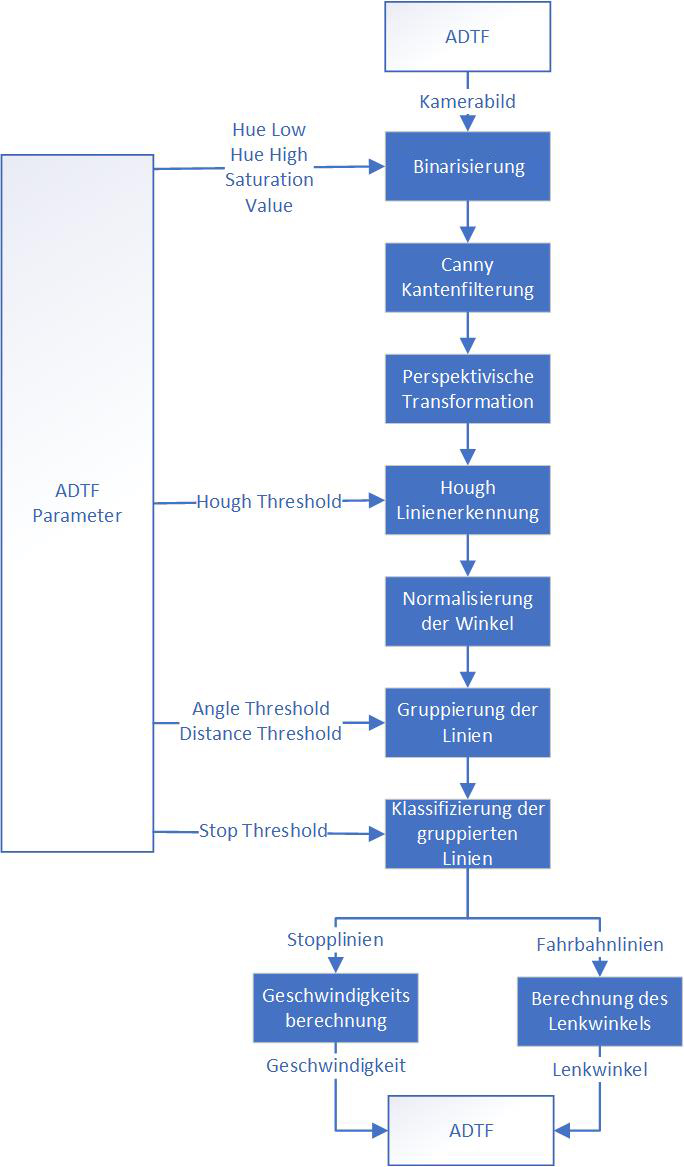
\includegraphics[width=.6\textwidth,keepaspectratio]{assets/bvaFlowchart.jpg}
		\caption{Übersicht der Bildverarbeitung}
		\label{img-bvaFlowchart}
	\end{figure}

\pagebreak

\section{Linienerkennung (Binarisierung)}
% Author: Frauke Jörgens
	Die von einer Kamera (RealSense\texttrademark\ oder der Basler-Kamera) aufgenommene RGB-Bilder werden zunächst in das HSV-Farbmodell übertragen, um eine genauere Segmentierung anhand von Farben im Bild zu ermöglichen, anstatt nur anhand der typischen Kanäle Rot, Grün und Blau des RGB-Farbmodells Farbbereiche zu erkennen.
	In dem HSV-Farbmodell werden Farben als Farbwinkel (0\degree\ für Rot, 120\degree\ für Grün, 240\degree\ für Blau \cite{HSV-Wiki}) repräsentiert. Zusätzlich wird die Sättigung und der Helligkeitswert der Farbe angegeben.
	Dieses Farbmodell erlaubt eine bessere -- und für Menschen intuitive -- Unterteilung von Farben im Bild.
	Da die Fahrbahnmarkierung aktuell blau ist, wird der blaue Anteil von den anderen Farben im Bild getrennt\footnote{Da es sich bei dem Bild um ein 8-Bit-Bild handelt, werden die Werte für den Farbwinkel (\textit{hue}) in den Bereich von 0\degree\ bis 180\degree\ skaliert, da Werte über 255 nicht über 8 Bit repräsentiert werden können.
	Siehe auch \url{https://docs.opencv.org/2.4/modules/imgproc/doc/miscellaneous_transformations.html\#cvtcolor} unter RGB $\longleftrightarrow$ HSV.}.
	Die zugehörigen Parameter (\texttt{hue}, \texttt{saturation} und \texttt{value}), die einen Unterraum des Farbraums bestimmen, können während der Laufzeit über die Eigenschaften des Filters in ADTF geändert werden, sodass auch Fahrbahnmarkierungen anderer Farben erkannt werden können.
	Die für uns idealen Parameter für das blaue Klebeband sind in \autoref{table-hsv-values} aufgeführt.

	\begin{table}
		\centering
		\begin{tabular}{r@{\,/\,}l|r@{$-$}l}
			Hue & Farbton & 90 & 120\\\hline
			Saturation & Sättigung & 100 & 255\\\hline
			Value & Helligkeitswert & 80 & 255
		\end{tabular}
		\caption{Gut funktionierende Parameter für die blaue Fahrbahnmarkierung. In ADTF werden \texttt{HueLow}, \texttt{HueHigh} und die unteren Grenzen für Sättigung (\texttt{Saturation}) und Helligkeitswert (\texttt{Value}) gesetzt.}
		\label{table-hsv-values}
	\end{table}

	Das Ergebnis dieser Operation ist ein Binärbild es unterteilt die Pixel des HSV-Bilds in Pixel, die Teil des Unterraums sind (weiß) und solche, die nicht Teil des Unterraums sind (schwarz).
	Für die Bestimmung der Unterräume sowie die Binarisierung wird die OpenCV-Funktion \texttt{cv::inRange} genutzt.
	Damit potenzielle Löcher, die durch Rauschen entstehen können, geschlossen werden, wird ein Closing auf das Binärbild angewandt.
	\autoref{img-applying-cvtColor} verdeutlicht die Anwendung dieser Bearbeitungsschritte.

	\begin{figure}
		\centering
		\begin{subfigure}[c]{0.45\textwidth}
			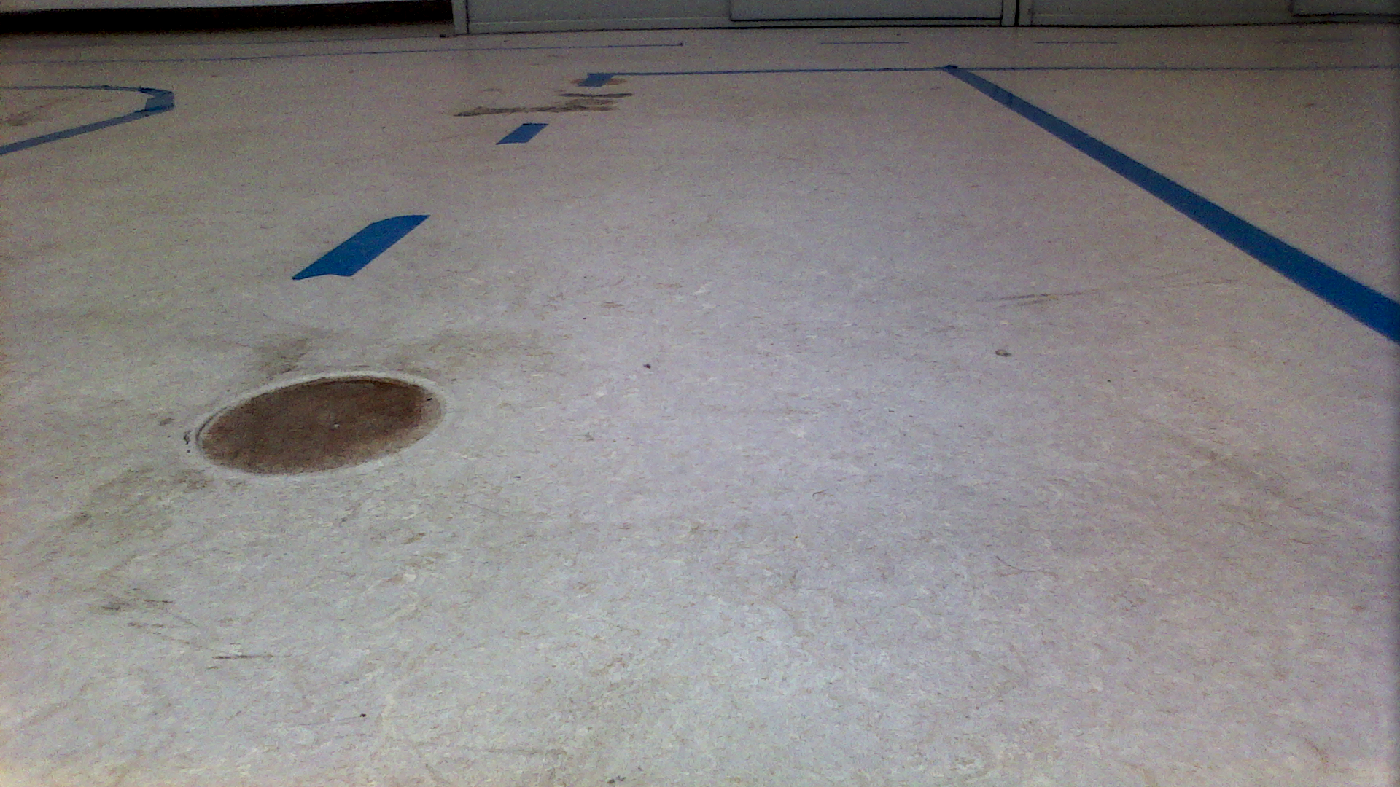
\includegraphics[width=\textwidth]{assets/Strasse.png}
		\end{subfigure}
		\begin{subfigure}[c]{0.45\textwidth}
			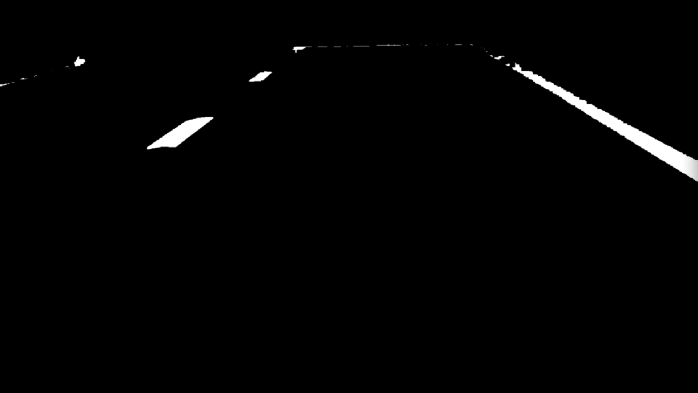
\includegraphics[width=\textwidth]{assets/Strasse-Binaer.png}
		\end{subfigure}
		\caption{Ursprüngliches Kamerabild der Realsense-Kamera (links) und binarisiertes Bild (rechts).}
		\label{img-applying-cvtColor}
	\end{figure}

\section{Canny Edge Detection}
% Author: Frauke Jörgens
	Um in dem Binärbild die Fahrbahnen als Linien erkennen zu können, wird ein Kantendetektionsverfahren -- der Canny Edge Detector, der bereits in OpenCV implementiert wurde -- verwendet\footnote{siehe auch \url{https://docs.opencv.org/2.4/doc/tutorials/imgproc/imgtrans/canny\_detector/canny\_detector.html}}.
	Dieser erkennt in einem Grauwertbild mithilfe des Sobel-Operators Kanten, deren Stärke und Gewichtung pro Pixel aufgenommen wird.
	Um sicherzustellen, dass die Kanten nur einen Pixel breit sind, werden alle zu Kanten zugehörigen Pixel, die keine lokalen Maxima sind, aussortiert.
	Schließlich werden über zwei Schwellenwerte die Kantenkandidaten weiter gefiltert, sodass ein Binärbild entsteht.
	Ist die Kantenstärke eines Pixels größer als der obere Schwellenwert, wird der Pixel als Kante akzeptiert.
	Ist die Kantenstärke eines Pixels niedriger als der untere Schwellenwert, wird dieser Pixel als Kandidat verworfen.
	Über eine Hysterese werden die Pixel gefiltert, die zwischen beiden Schwellenwerten liegen, sodass "`Ausreißer"' vermieden werden.

	Dementsprechend nimmt die Funktion \texttt{cv::Canny}, bzw. das GPU-Pendant \texttt{cv::cuda::createCannyEdgeDetector} in Kombination mit der Funktion \texttt{detect}, die auf das Objekt angewandt wird, neben dem Bild folgende Parameter entgegen: \texttt{threshold1}, der die untere Grenze für die Aussortierung der Kandidaten bildet, \texttt{threshold2}, der die obere Grenze für die Aussortierung der Kandidaten bildet und \texttt{apertureSize}, die Größe des Sobel-Operators.
	Für das Verhältnis der Schwellenwerte zueinander wird das Verhältnis 2:1 bzw. 3:1 (\textit{upper:lower}) empfohlen.
	\autoref{img-applying-canny} zeigt das Ergebnis des Canny-Algorithmus' nach der Anwendung auf das Binärbild.
	% NOTE: Das ist okay, aber ihr dürft davon ausgehen, dass der Leser weiß, wie der Canny Filter arbeitet. Ihr müsst die Parameter nicht erklären, es sei denn das war euch bei der Parameterwertsuche besonders wichtig. Konzentriert euch lieber auf die Beschreibung von dem, was ihr gemacht habt. :) --hoe

	\begin{figure}
		\centering
		\begin{subfigure}[c]{0.45\textwidth}
			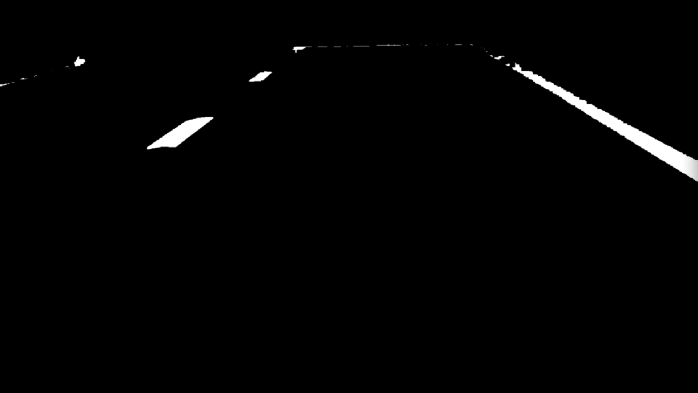
\includegraphics[width=\textwidth]{assets/Strasse-Binaer.png}
		\end{subfigure}
		\begin{subfigure}[c]{0.45\textwidth}
			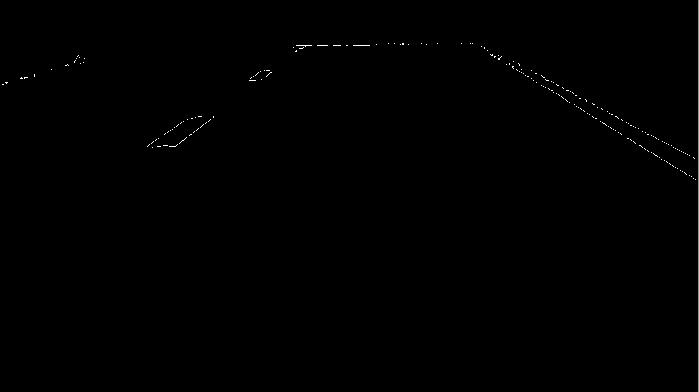
\includegraphics[width=\textwidth]{assets/Strasse-Canny.png}
		\end{subfigure}
		\caption{Kamerabild vor (links) und nach der Anwendung des Canny-Algorithmus' (rechts).}
		\label{img-applying-canny}
	\end{figure}

\section{Perspektivische Verzerrung}
% Author: Frauke Jörgens
	Die Realsense-Kamera, die genutzt wird, sieht die Straße in einem Winkel, der nicht im rechten Winkel zur Straße ist.
	Daraus ergibt sich eine perspektivische Verzerrung, die im Kamerabild deutlich wird.
	Für die Bildverarbeitung wäre allerdings ein orthografisch projiziertes Bild (ähnlich der Vogelperspektive) ideal, um Probleme, die aufgrund der Perspektive auftreten, zu vermeiden.
	Beispielsweise erhofften wir uns von diesem Ansatz, Kurven besser erkennen zu können.

	Anhand eines Schachbrettmusters wurde das Kamerabild so kalibriert, dass die Quadrate des Musters auch im Kamerabild quadratisch sind.
	Zur Transformation werden 4 Punkte benutzt, die ein Viereck aufspannen und die Eckpunkte der Straße angeben. Anhand der OpenCV-Funktion \texttt{cv::get\-PerspectiveTransform} wird die zugehörige Transformationsmatrix berechnet, welche mit der OpenCV-Funktion \texttt{cv::cuda::warpPerspective} angewandt wird. \autoref{img-applying-persp-warp} zeigt das Bild der Straße vor und nach Anwendung der perspektivischen Verzerrung.

	\begin{figure}[h]
		\centering
		\begin{subfigure}[c]{0.45\textwidth}
			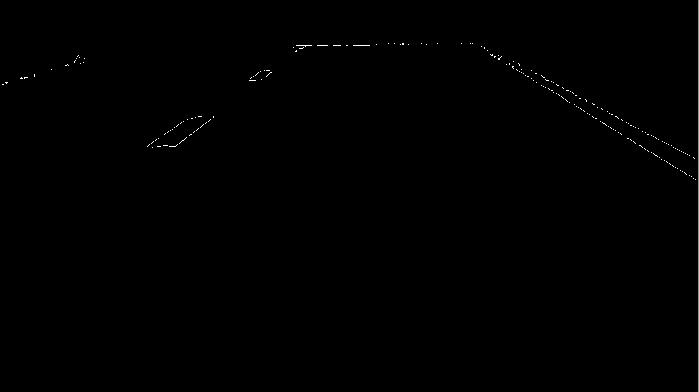
\includegraphics[width=\textwidth]{assets/Strasse-Canny.png}
		\end{subfigure}
		\begin{subfigure}[c]{0.45\textwidth}
			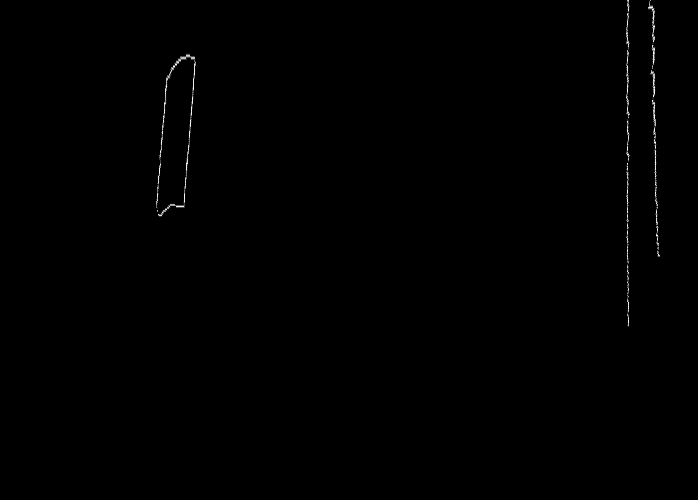
\includegraphics[width=.8\textwidth]{assets/Strasse-Persp.png}
		\end{subfigure}
		\caption{Kamerabild vor (links) und nach der Anwendung der perspektivischen Verzerrung (rechts).}
		\label{img-applying-persp-warp}
	\end{figure}

\section{Hough Line Transformation}
% Author: Jan Ottmüller

	Nachdem die Kanten der Fahrbahnen nun gefiltert sind, können aus den Bilddaten die Fahrstreifen abstrahiert werden.
	Für die Positionsberechnung ist es notwendig, die Fahrbahnen nun in dem gefilterten Bild zu erkennen, und in geeigneter Weise mathematisch zu repräsentieren.

	OpenCV bringt die hierfür geeignete Hough Line Transformation mit.
	Diese transformiert das Bild in den Hough Raum.
	Über einen Threshhold Parameter kann hierbei die Empfindlichkeit des Filters eingestellt werden.
	Je niedriger, desto mehr Linien werden im Bild erkannt.
	Diesen Parameter kann im ADTF zur Laufzeit angepasst werden.

	Ebenfalls probierten wir zu Anfang noch die probabilistic Hough Transformation aus.
	Diese, ebenfalls von OpenCV mitgebrachte Funktion, hat die zusätzliche Eigenschaft, dass beispielsweise die gestrichelten Mittellinien nicht als eine einzelne Gerade erkannt werden, sondern jeder Strich der Mittellinie als einzelne Gerade.
	Da uns jedoch nur die Mittellinie an sich interessiert, haben wir uns dazu entschieden, diese Transformation nicht zu verwenden.
	Dies reduziert zudem die Menge der zu verarbeitenden Geraden.

	Die mit Hilfe der Hough Line Transformation erkannten Geraden werden in Polarkoordinaten dargestellt.
	Hierbei befindet sich der Ursprung oben links im Bild.
	Von diesem Punkt aus wird die Gerade mit einem orthogonalen Stützvektor mit dem Winkel $\theta$ und der Länge $r$ beschrieben (siehe auch \autoref{img-Winkelnormalisierung}).

\section{Winkelnormalisierung}
% Author: Frauke Jörgens

	Bevor die Linien zusammengefasst werden, werden sie einer Normalisierung unterzogen.
	In OpenCV haben die Normalenvektoren, die sich nach der Hough Line Transformation ergeben, einen Winkel von $0$ bis $180\degree$ zu der x-Achse.
	Bei einem theoretisch größeren Winkel wird die Gerade durch eine negative Distanz dargestellt.
	Da vertikale Linien einen horizontalen Normalenvektor haben, schwanken die Winkel oft zwischen $\sim0$ und $\sim180\degree$ bei vertikaler Ausrichtung.
	
	In dem Straßenbild sind oft vertikale Linien vorhanden.
	Um die Erkennung dieser einfacher zu machen, werden die Winkel der gefundenen Linien so verändert, dass sie in einem Bereich von -90 bis +90 $\degree$ liegen.
	Vertikale Linien haben folglich einen Winkel von ca. $0 \degree$.
	Winkel außerhalb dieses Bereichs werden anhand einer negativen Distanz dargestellt.
	Aufgrund der Tatsache, dass das Bild so verzerrt wurde, dass wir die Straße aus einer senkrechten Obersicht betrachten, entsprechen die Winkel der gefunden Geraden nun dem relativen Winkel der Fahrbahn zur Fahrtrichtung.
	\autoref{img-Winkelnormalisierung} verdeutlich diese Überlegung.
	
	\begin{figure}
		\centering
		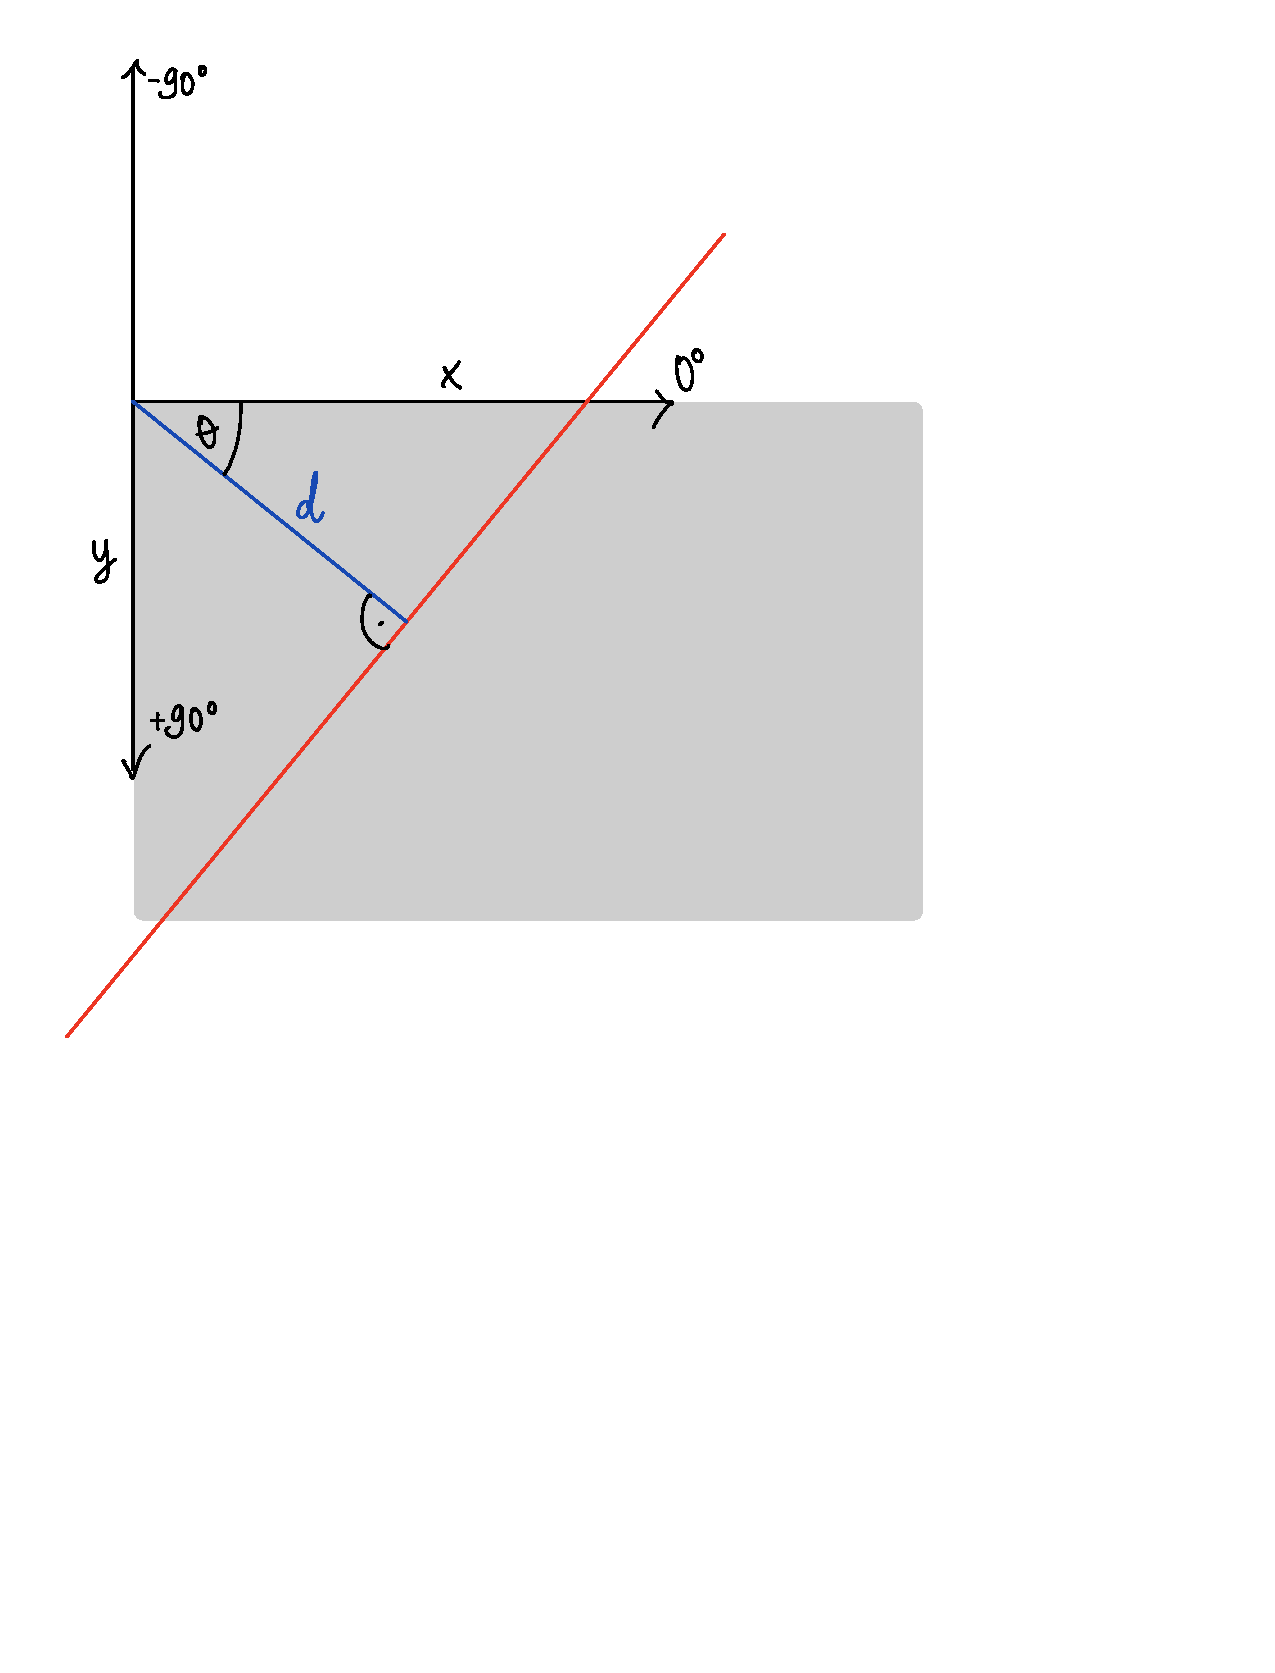
\includegraphics[height=0.5\textheight]{assets/Winkelnormalisierung.pdf}
		\caption{Darstellung des Winkels anhand eines Beispiels}
		\label{img-Winkelnormalisierung}
	\end{figure}

\section{Line-Clustering}
% Author: Frauke Jörgens
	Durch die Hough Line Transformation werden tendenziell zu viele Linien gefunden.
	Um die Anzahl der Linien zu reduzieren, wird ein Clustering mithilfe der Funktion \texttt{cv::partition} verwendet, welches die Linien in Äquivalenzklassen unterteilt.
	Es wird eine Äquivalenzfunktion benutzt, die besagt, wann zwei Linien als äquivalent angesehen werden (im Quellcode \texttt{isEquivalent} genannt).
	Der Vergleich erfolgt anhand des Winkels und der Länge des Normalenvektors der Linie.
	Nach dem Clustering ist jede Linie einer Klasse zugeordnet.
	Alle Linien einer Klasse werden anschließend zu einer Linie zusammengefasst, indem Winkel und Abstand der Klasse zugehörigen Linien gemittelt werden.
	Zusätzlich wird für jede zusammengefasste Linie gespeichert, aus wie vielen Linien sie zusammengefasst wurde, um anhand dessen eine Gewichtung zu ermöglichen.

\section{Klassifizierung}
% Author: Frauke Jörgens
	Nachdem die Linien aufgrund des Ähnlichkeitskriteriums gebündelt wurden, werden sie in Kategorien unterteilt, um das Straßenbild sinngemäß zusammenzufassen.
	Wir haben uns für eine Unterteilung in Kategorien entschieden, die in \autoref{table-lineClassification} aufgelistet und beschrieben sind. %NOTE: Wirkt etwas gedrungen. Vielleicht lieber Aufzählung? --felix
	\begin{table}
		\begin{tabular}{p{.125\textwidth}|p{.35\textwidth}|p{.35\textwidth}|p{.05\textwidth}}
			Art der Linie & Beschreibung & Bedingung & Farbe\\\hline
			Linke Linie &  Die linke erkannte Linie. Aufgrund des Kamerablickwinkels entspricht diese Linie also eigentlich der mittleren gestrichelten Linie der Straße & Die Linie ist vertikal (ihr Winkel zur y-Achse ist kleiner als 20\degree) und sie befindet sich auf der linken Seite des Bildes & grün\\\hline
			Rechte Linie & Die rechte erkannte Linie (= die rechte Fahrbahnmarkierung) & Die Linie ist vertikal (s.o.) und sie befindet sich auf der rechten Seite des Bildes & blau\\\hline
			Haltelinie & Eine Haltelinie, wie sie an einer Kreuzung üblich ist & Die Linie ist horizontal (ihr Winkel zur y-Achse ist größer als 75 \degree) & rot\\\hline
			Unklassifi-zierte Linie & Eine Linie, die keiner der obigen Kategorien entspricht & Eine Linie wird keiner der Kategorien zugeordnet  & gelb\\
		\end{tabular}
		\caption{Beschreibung der verschiedenen Klassen von erkannten und nicht erkannten Linien.
		In \autoref{img-lines} wird veranschaulicht, wie die Linien entsprechend ihrer Klasse eingefärbt und anhand der Anzahl der zusammengefassten Linien dicker oder dünner gezeichnet werden.}
		\label{table-lineClassification}
	\end{table}

	\begin{figure}
		\centering
		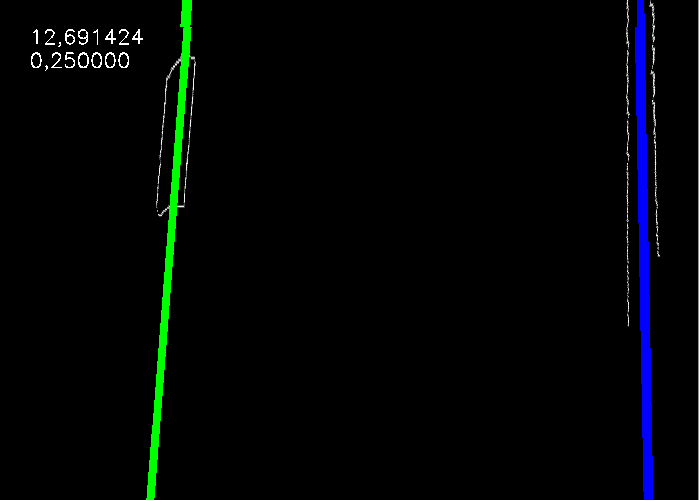
\includegraphics[width=.5\textwidth]{assets/Strasse-Final}
		\caption{Perspektivisch verzerrtes Canny-Bild aus \autoref{img-applying-persp-warp} mit erkannten Linien.
			Es wurde eine Linke (grün) und eine Rechte (blau) erkannt. Oben links im Bild wird der berechnete Lenkwinkel und die berechnete Geschwindigkeit angezeigt.}
		\label{img-lines}
	\end{figure}

% TODO vllt noch ein Bild mit erkannter Stopplinie und unklassifizierten Linien am Montag machen?

\subsection{Haltelinien}
% Author: Jan Ottmüller

	Wird eine waagerechte Linie erkannt, so wird sie als Haltelinie klassifiziert.
	Je näher sich das Fahrzeug dieser Linie nähert, desto langsamer wird es.
	Dieser Anhaltealgorithmus ist jedoch nur aktiv, wenn genügend Haltelinien bzw. eine stark gewichtete Haltelinie erkannt wurden.
	So vermeiden wir, dass das Auto schon anhält, wenn es nur eine sehr schwache Stopplinie erkannt hat, was durch Rauschen ausgelöst werden kann.
	Dieser Schwellenwert kann mit dem ADTF-Parameter 'Stop Threshold' angepasst werden.
	Für uns hat der Wert 0,4 gut funktioniert.
	Es müssen dann also mindestens 40\% der Linien eine Stopplinie sein, damit das Fahrzeug anhält. %NOTE: Ist das wirklich so? -- felix

\section{Zentrierung in der Fahrspur}
% Author: Felix Maaß

	Bisher ist das Auto in der Lage der Fahrspur zu folgen.
	Allerdings besteht das Problem, dass es sich nicht in der Mitte der Spur zentriert.
	Dies führt dazu, dass es oft bereits auf den Linien fährt und teilweise sogar die andere Fahrspur mitbenutzt.
	Da es sich hierbei um unerwünschtes Verhalten handelt, thematisiert dieser Abschnitt unsere Herangehensweise.

\subsection{Theoretische Überlegungen}
% Author: Felix Maaß

	Angenommen es werden zwei Linien (linke und rechte Leitlinie) erkannt.
	Es wird nun jeweils der Abstand zur Seite ermittelt und dann gemittelt (Arithmetisches Mittel).
	Das Ergebnis ist ein Wert, der entweder links, rechts oder genau auf der Ideallinie des Fahrspur liegt.

	Es wird nun eine Funktion gesucht, die die Abweichung in eine Lenkanweisung umsetzt.
	Da dies schnell zu instabilem Verhalten führen kann, fällt eine lineare Funktion raus.
	Hier würde zu oft nachkorrigiert werden müssen.

	Unsere Wahl fiel daher auf eine modifizierte Sigmoid-Funktion:

		\[y=\frac{a_{max}}{1 + e^{-14\left( \frac{\left\|x\right\|}{x_{max}} - \frac{1}{2} \right)}} \cdot -\frac{x}{\left\|x\right\|}\]

	Hierbei steht $x$ für die aktuelle und $x_{max}$ für die maximale Abweichung von der Ideallinie.
	Der maximal anzusteuernde Lenkwinkel wird durch den Parameter $a_{max}$ angegeben.

	\paragraph{Veranschaulichung.} \autoref{img-spurzentrierung-function} zeigt die Funktion beispielhaft für eine maximale Abweichung von $x_{max} = 100mm$ und die damit einhergehende maximale Lenkwinkelreaktion von $a_{max} = 20\degree$.

	Je weiter sich das Auto von der Ideallinie entfernt, desto stärker wird der Lenkeinschlag und somit der Drang sich wieder zu zentrieren.

	Durch das exponentielle Verhalten ist sichergestellt, dass ein Aufschwingen unwahrscheinlich ist. Dies begründen wir dadurch, dass die Amplifikation um den Nullpunkt so gering ist, dass sie in der Praxis wie eine Totzone wirkt.

	\begin{figure}[ht]
		\centering

		\begin{tikzpicture}
		\datavisualization [
		scientific axes=clean,
		style sheet=strong colors,
		style sheet=vary dashing,
		all axes={grid}, scale=2,
		y axis={label=Lenkwinkel, ticks={few, tick unit=\degree}},
		x axis={label=Abweichung, ticks={step=50, tick unit=mm}},
		visualize as smooth line,
		data/format=function
		]

		data {
			var x : interval [-100:100] samples 20;
			func y = 20 / (1 + e^(-14 * (abs(\value x)/100 - 1/2))) * -\value x / abs(\value x);
		};
		\end{tikzpicture}

		\caption{Spurzentrierung mit $a_{max} = 20\degree$ und $x_{max} = 100mm$}
		\label{img-spurzentrierung-function}
	\end{figure}

\section{Besonderheiten in der Kurve}
% Author: Frauke Jörgens
% TODO (macht Frauke)
	

\section{Weitere Überlegungen}
% Author: Jan Ottmüller

	An dieser Stelle möchten wir noch einige Überlegungen und Erkenntnisse festhalten,
	die es nicht in die fertige Software geschafft haben.

\subsection{Alternative Fahrstreifenrepräsentation}

	In den Anfängen der Implementierung entschieden wir uns dafür, die Fahrstreifen durch Geraden zu repräsentieren und aus diesen den Lenkwinkel zu berechnen.
	Hierdurch können gerade Fahrstreifen sehr präzise dargestellt werden, jedoch zeigt das Verfahren Schwächen bei der Repräsentation von Kurven.
	Eine andere Form der Darstellung wäre eine Polynomfunktion zweiten Grades.
	Hierbei kann die Polynomfunktion genau an die Kurve angepasst werden.
	Da unser erster Ansatz jedoch schon recht gut funktionierte und wir keine geeignete Funktion für das Anpassen der Polynomfunktion fanden, haben wir uns auf unseren schon implementierten Ansatz weiter konzentriert.

%%%%%%%%%%%%%%%%%%%%%%%%%%%%%%%%%%%%%%%%%%%%%%%%%%
\chapter{Aggregation und Interpretation von Erkenntnissen}

	Zuletzt werden alle Ergebnisse aus den vorgeschalteten Filtern zusammengeführt und eine finale Entscheidung getroffen, welche Aktionen durchgeführt werden sollen.
	Dazu wurde der \texttt{cMainController} entwickelt. Er nimmt nun den Lenkwinkel und die Geschwindigkeit der Fahrbahnerkennung sowie die Flags der Hindernis- und Kollisionserkennung entgegen und evaluiert darauf basierend die aktuelle Lage.

	Der Filter steuert dann die Geschwindigkeit und den Lenkwinkel sowie die Fahrzeugbeleuchtung.

	Grob gesagt, wird hier zwischen den folgenden Verhalten differenziert:

	\begin{enumerate}
		\item{\textbf{Normaler Zustand: Fahrt}
			\begin{enumerate}
				\item Lenkwinkel und Geschwindigkeit werden durchgereicht.
				\item Abblendlicht ist eingeschaltet. Bremslicht ist optional aktiv.
			\end{enumerate}
		}
		\item{\textbf{Normaler Zustand: Haltelinie erkannt}\footnote{Ein- und Ausgänge für das Verhalten an Kreuzungen (wie ``In welche Richtung soll abgebogen werden?'') sind bereits mit eingeplant und sind auch in Verwendung. Allerdings unterstützen die folgenden Filter diese Aktionen noch nicht.}
			\begin{enumerate}
				\item Es wird eine Aktion ausgewählt (wie z.B. \emph{rechts abbiegen}).
				\item Abblendlicht ist eingeschaltet. Bremslicht ist aktiv.
			\end{enumerate}
		}
		\item{\textbf{Gefahren-Zustand: Hindernis erkannt}
			\begin{enumerate}
				\item Der letzte Lenkwinkel wird beibehalten und die Geschwindigkeit auf $0$ gesetzt.
				\item Zusätzlich zum Abblend- und Bremslicht ist auch der Warnblinker eingeschaltet.
			\end{enumerate}
		}
		\item{\textbf{Gefahren-Zustand: Kollision erkannt}
			\begin{enumerate}
				\item Der letzte Lenkwinkel wird beibehalten und die Geschwindigkeit auf $0$ gesetzt.
				\item Zusätzlich zum Abblend- und Bremslicht ist auch der Warnblinker eingeschaltet.
			\end{enumerate}
		}
	\end{enumerate}

	Zwischen den ersten drei Zuständen wird automatisch gewechselt.
	Ist jedoch eine Kollision erkannt worden, verweilt der Controller solange in diesem Zustand, bis er durch einen Eingriff des Menschen über die Filtereigenschaften zurückgesetzt wird.

%%%%%%%%%%%%%%%%%%%%%%%%%%%%%%%%%%%%%%%%%%%%%%%%%%
\chapter{Modifikationen am Fahrzeug}

Damit die Kamera in einem besseren Winkel auf die Straße blickt, haben wir sie weiter vorne am Modellauto mit einer 3D-gedruckten Halterung befestigt. Um die Kamera wieder an ihrer ursprünglichen Position zu befestigen, muss sie oben mit dem Magneten und mit einer Schraube mit 3 Unterlegscheiben gesichert werden.
\begin{figure}[ht]
	\centering
	\begin{subfigure}[c]{.45\textwidth}
		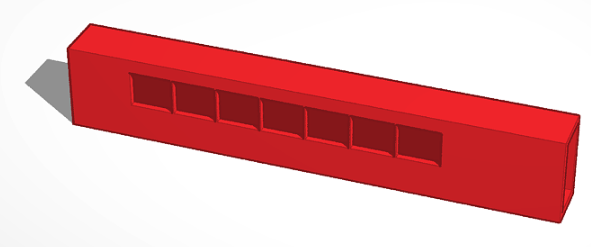
\includegraphics[width=\textwidth]{assets/Kamerahalterung.PNG}
	\end{subfigure}
	\begin{subfigure}[c]{.45\textwidth}
		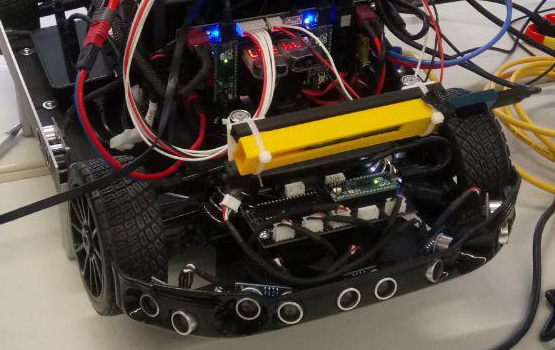
\includegraphics[width=\textwidth]{assets/Kamera-Anbringung.jpg}
	\end{subfigure}
	\caption{CAD-Modell der Halterung (links) und Anbringung des 3D-Modells (gelb) und der Kamera am Modellfahrzeug (rechts).}
	\label{img-camera}
\end{figure}


\chapter{Fazit}
%- lange noch nicht fertig
%- viele interessante theoretische Ansätze, die noch nicht umgesetzt wurden
%- Einarbeitung in ADTF unterschätzt
%- ADTF generell "schickes" Konzept/Design -> Umsetzung eher zu Lasten der Usability + manchmal fragwürdige Entscheidungen der Entwickler (void * statt Generics, viele Fehler in dem Code von Audi)
%- Dokumentation im Code teilweise falsch (noch schlimmer als keine)
%- vllt Abstürze erwähnen
%- Vllt wäre in der BVA der Ansatz mit den Polynomfunktionen besser gewesen
%- Zu Lenkng \& Motorregelung: Theorie != Praxis, Schlupf der Räder, Rauschen in Messwerten erschwerten den Umgang (ließen theoretische Überlegungen vollkommen von der Praxis abweichen)
%- Bei Beschleunigungssensor schwer zu unterscheiden, ob absichtliches Bremsen oder gegen weiches Objekt fahren, oder Erschütterungen im Boden
% TODO Fazit hier!

\listoftables

%%%%%%%%%%%%%%%%%% BIBLIOGRAPHY %%%%%%%%%%%%%%%%%%

\begin{thebibliography}{9}

	\bibitem{hoffmann_ws17}
	Prof. Dr. Ulrich Hoffmann,
	\textit{Einführung in die Robotik},
	Fachhochschule Wedel - Wintersemester 2017/18:\\
	\url{http://www.fh-wedel.de/mitarbeiter/uh/lehrveranstaltungen/ws1718/einfuehrung-in-die-robotik/}

	\bibitem{Regelungstechnik}
	Prof. Dr.-Ing. Carsten Burmeister,
	\textit{Regelungstechnik},
	Fachhochschule Wedel - Wintersemester 2017/18

	\bibitem{berry16}
	Nick Berry,
	\textit{Ackerman Steering},
	December 2016:\\
	\url{http://datagenetics.com/blog/december12016/index.html}

	\bibitem{HSV-Wiki}
	Wikipedia,
	\textit{HSV-Farbraum}.\\
	Letzte Bearbeitung: 8. September 2017 um 17:55 Uhr,
	Letzter Zugriff am: 21. Januar 2018,
	\url{https://de.wikipedia.org/wiki/HSV-Farbraum}

\end{thebibliography}

\end{document}
